\thispagestyle{quantoannone}
\pagestyle{quantoan}
\everymath{\color{quantoan}}
\graphicspath{{../quantoan/pic/}}
\blfootnote{\color{quantoan}\color{quantoan}$^1$The Bizarre World of Nontransitive Dice: Games for Two or More Players. The College Mathematics Journal, Vol. $48$, No. $1$ (January $2017$), pp. 2 $- 9$.}
\begingroup
\AddToShipoutPicture*{\put(0,616){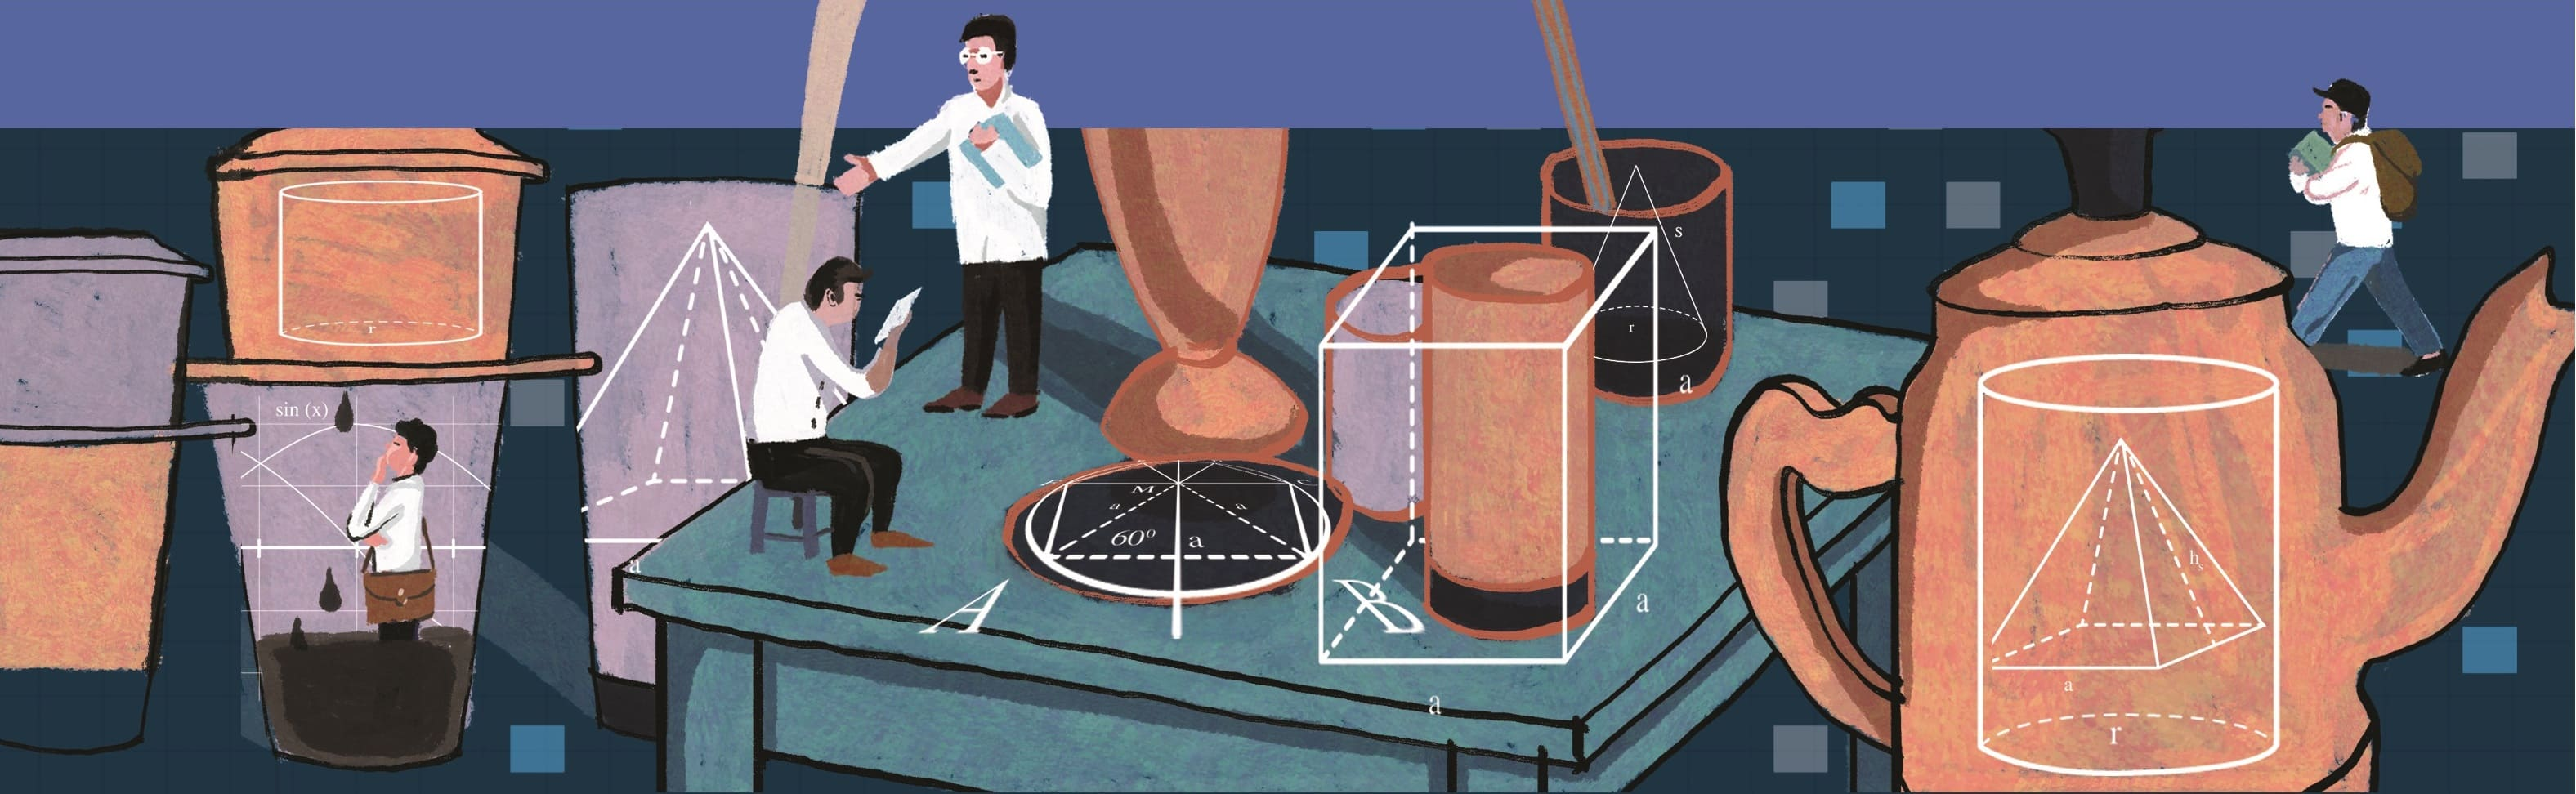
\includegraphics[width=19.3cm]{../bannerquantoan}}}
\AddToShipoutPicture*{\put(82,507){
\includegraphics[scale=1]{../tieude2.pdf}}}
\centering
\endgroup

\vspace*{202pt}

\begin{multicols}{2}
	\textit{Với những con xúc xắc không bắc cầu, bạn luôn có thể chọn một con xúc xắc có xác suất thắng lớn hơn con xúc xắc của đối thủ. Một số bộ ba và bộ bốn con xúc xắc không bắc cầu đã được biết đến rộng rãi. Trong bài viết này, chúng ta tìm cách tạo ra một bộ xúc xắc không bắc cầu cho phép thắng hai đối thủ cùng một lúc. Đã có một trò chơi ba người như vậy được thiết kế, với bảy con xúc xắc. Bằng cách khai thác tính đổi chiều của một số con xúc xắc, chúng tôi đưa ra một trò chơi ba người cải tiến với \linebreak năm con xúc xắc.}
	\vskip 0.05cm
	Bạn có thể rủ một người bạn chơi trò chơi sau đây. Đó là một trò chơi hai người, sử dụng ba con xúc xắc. Tuy nhiên, đây không phải là những con xúc xắc thông thường, bởi các giá trị trên mặt của chúng không phải là các số từ $1$ đến $6$.
	\vskip 0.05cm
	Trò chơi rất đơn giản: Mỗi người chọn và lăn một con xúc xắc, ai được nhiều điểm hơn thì~thắng.
	\vskip 0.05cm
	Trò chơi có vẻ khá cân bằng. Thế nhưng, trong một trò chơi, chẳng hạn, mười lượt, bạn luôn có thể chọn được một con xúc xắc có xác suất thắng lớn hơn, bất kể người bạn của bạn chọn con xúc xắc nào. Và bạn có thể tự làm những con xúc xắc này ở nhà.
	\vskip 0.05cm
	Trong hình dưới đây\footnote[2]{\color{quantoan}Chúng tôi giữ nguyên các tên màu bằng tiếng Anh trong hình vẽ, vì lý do sẽ được làm rõ ở phần sau của bài viết.} là một bộ ba con xúc xắc đặc biệt như thế:
	\begin{figure}[H]
		\vspace*{-5pt}
		\centering
		\captionsetup{labelformat= empty, justification=centering}
		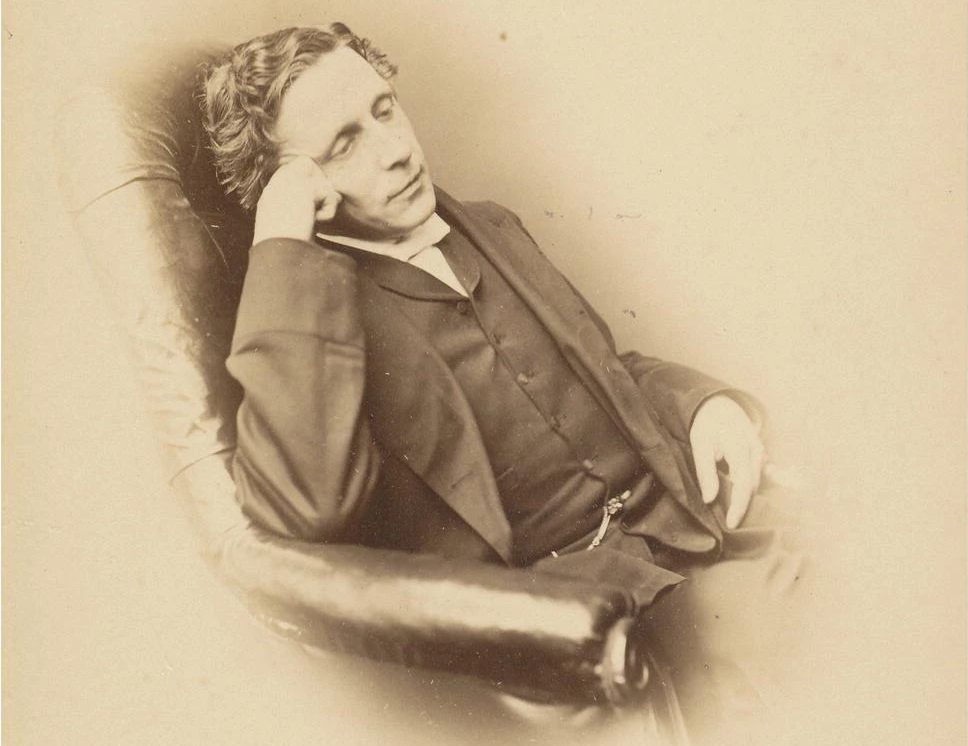
\includegraphics[width= 0.8\linewidth]{1}
%		\caption{\small\textit{\color{}}}
		\vspace*{-15pt}
	\end{figure}
	Ta nói con xúc xắc $A$ thắng con xúc xắc $B$ nếu xác suất để $A$ thắng $B$ lớn hơn $50\%$. Có thể dễ dàng chứng minh con xúc xắc Đỏ thắng con xúc xắc Xanh da trời bằng lược đồ cây dưới đây:
	\begin{figure}[H]
		\vspace*{-15pt}
		\centering
		\captionsetup{labelformat= empty, justification=centering}
		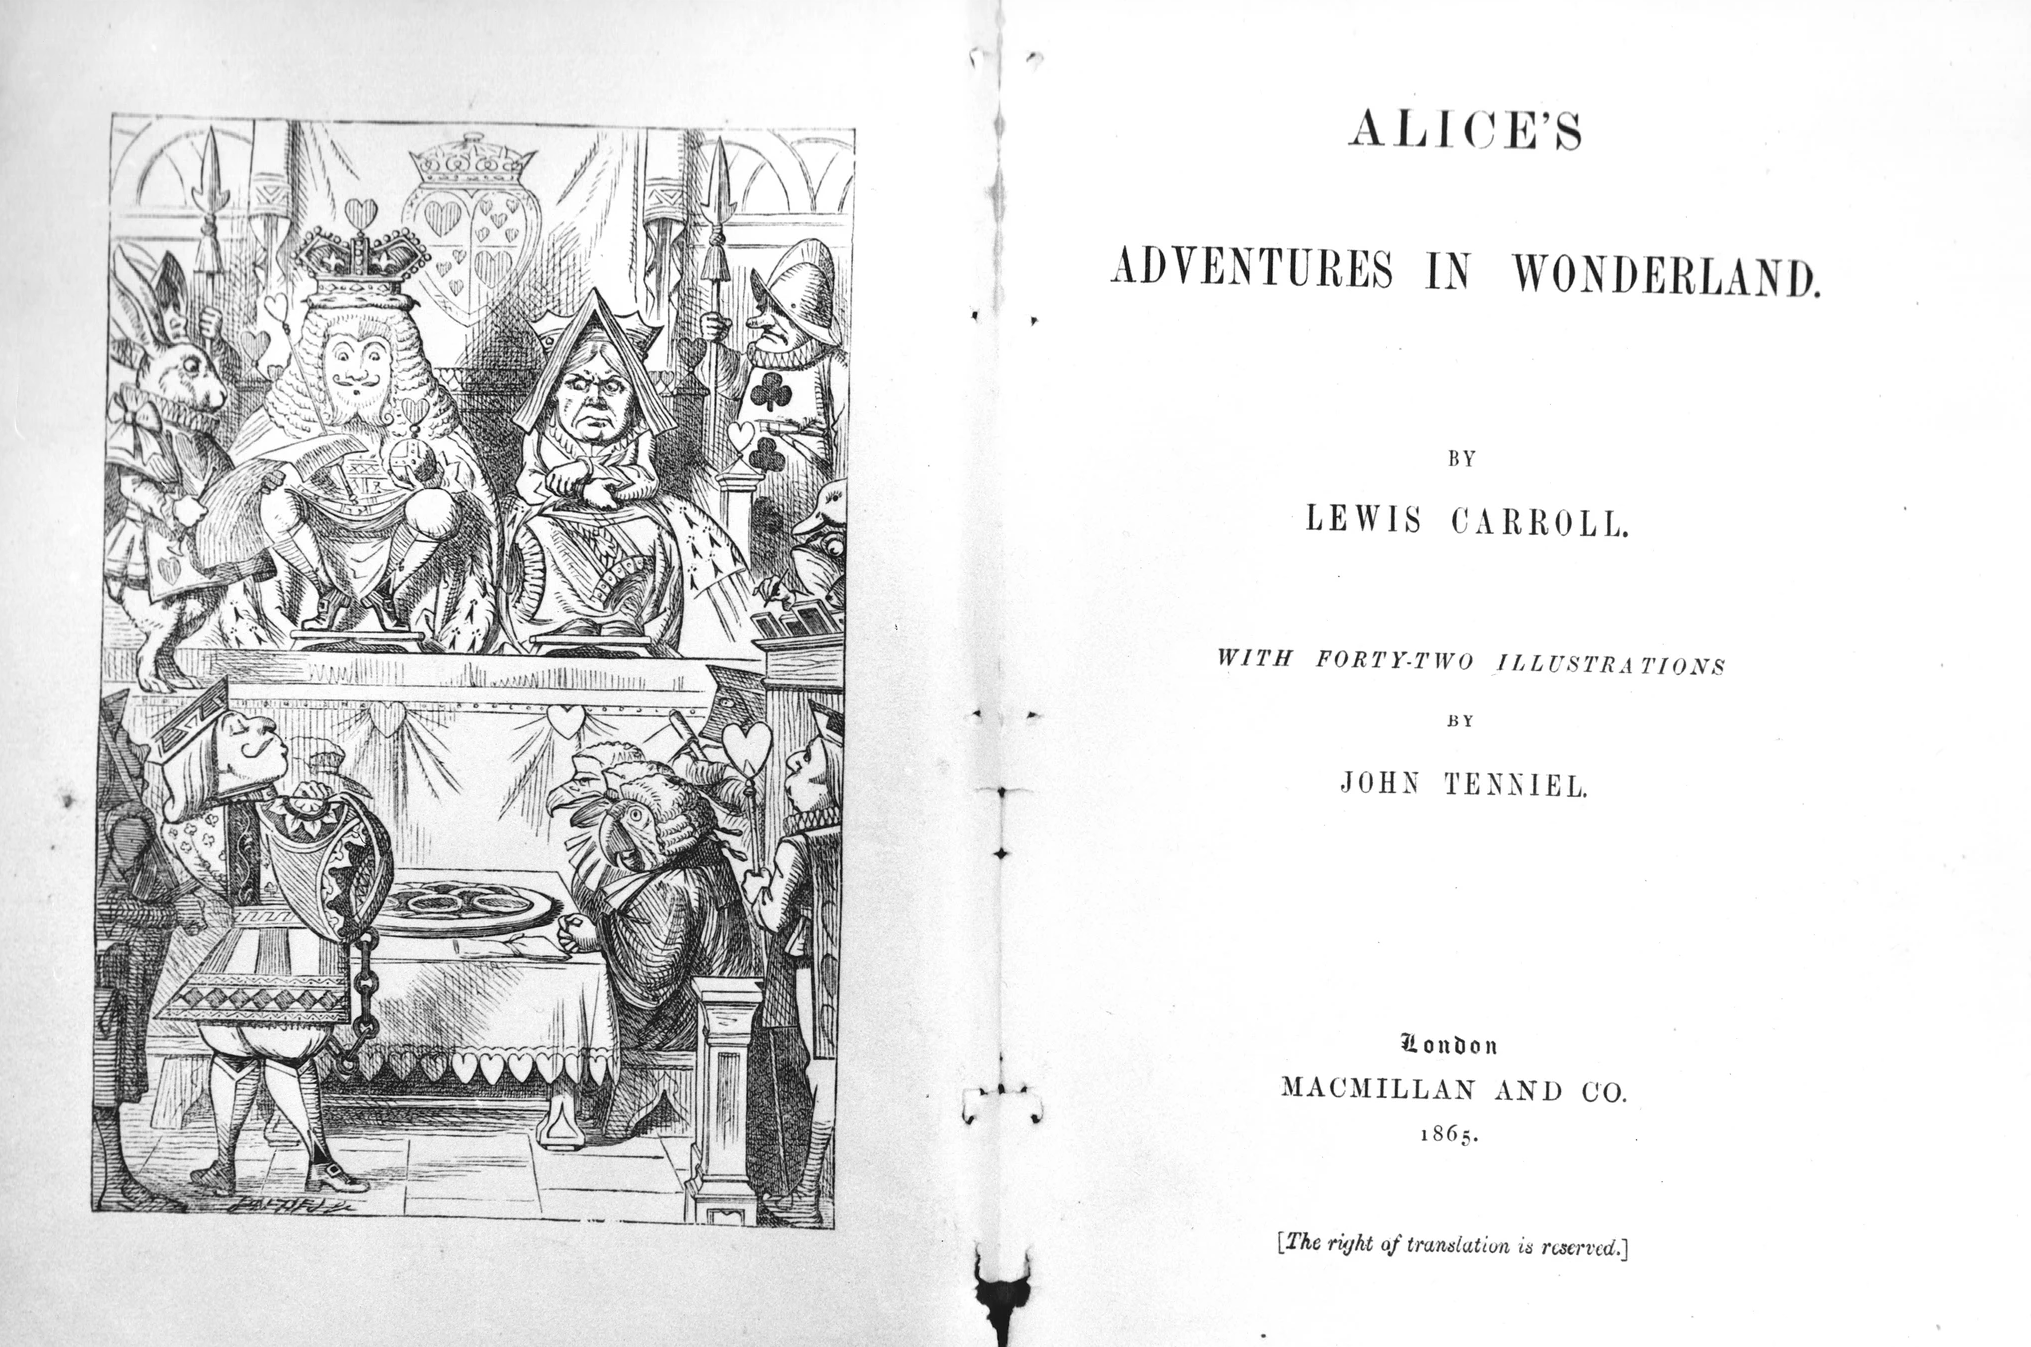
\includegraphics[scale =1]{2}
%		\caption{\small\textit{\color{}}}
		\vspace*{-15pt}
	\end{figure}
	Từ lược đồ cây, ta thấy Đỏ thắng Xanh da trời với xác suất $7/12$, vì vậy Đỏ là lựa chọn tốt hơn trong trường hợp này.
	\vskip 0.05cm
	Tương tự, ta có thể tính được xác suất để Xanh da trời thắng Xanh lá cây là $7/12$, từ đó thiết lập được một chuỗi quan hệ thắng bại trong đó Đỏ thắng Xanh da trời, Xanh da trời thắng Xanh lá cây.
	\begin{figure}[H]
		\vspace*{-10pt}
		\centering
		\captionsetup{labelformat= empty, justification=centering}
		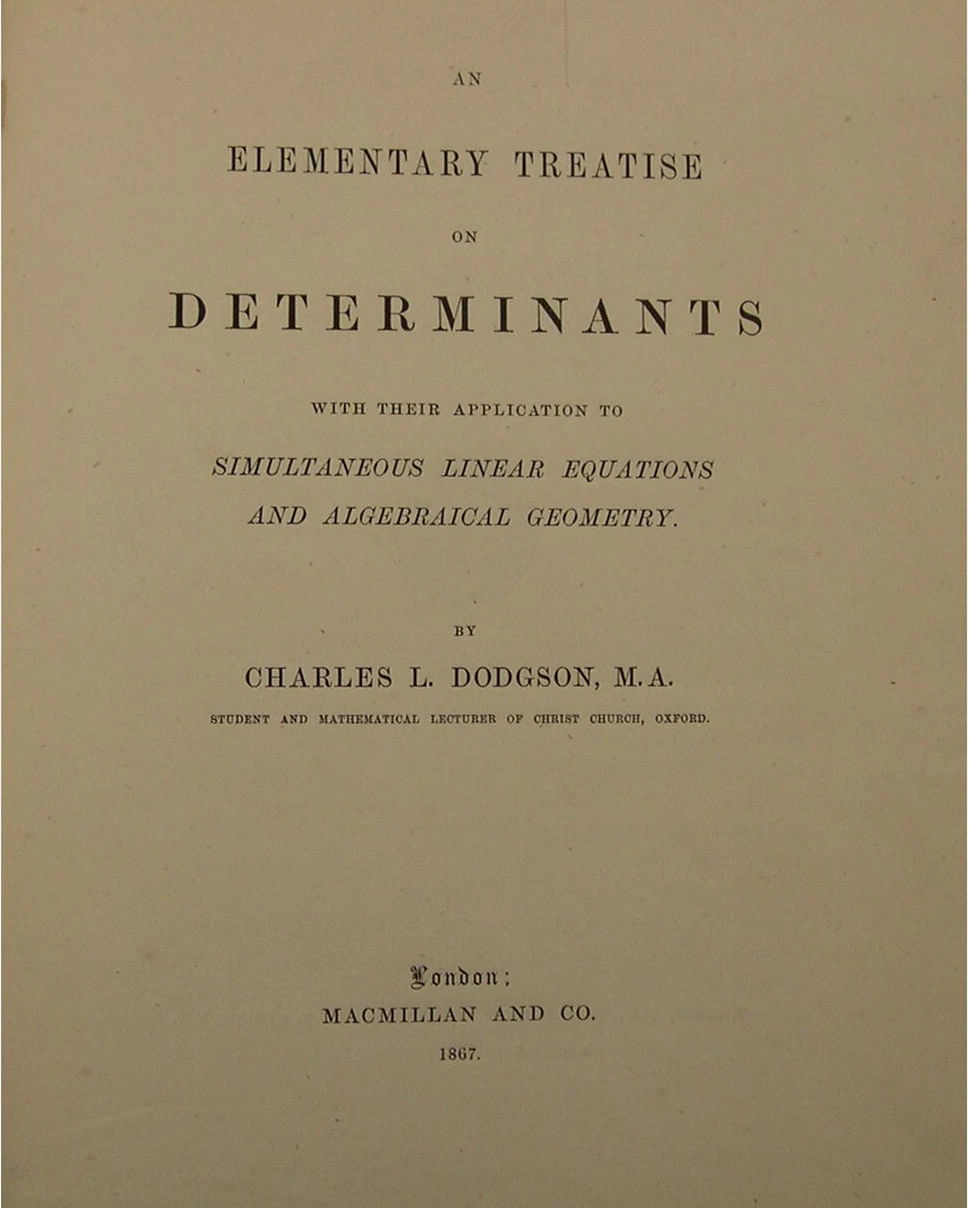
\includegraphics[scale =0.9]{3}
%		\caption{\small\textit{\color{}}}
		\vspace*{-15pt}
	\end{figure}
	Từ thông tin này, sẽ là hoàn toàn hợp lý khi kỳ vọng rằng Đỏ thắng Xanh lá cây. Nếu quả đúng như vậy, ta nói rằng các con xúc xắc này có tính bắc cầu.
	\vskip 0.05cm
	Thế nhưng điều đó lại không đúng. Kỳ quái làm sao, sự thực là Xanh lá cây lại thắng Đỏ với xác suất $25/36$. Nghĩa là chuỗi quan hệ thắng bại là một vòng tròn, giống như trò oẳn tù tì.
	\begin{figure}[H]
		\vspace*{-10pt}
		\centering
		\captionsetup{labelformat= empty, justification=centering}
		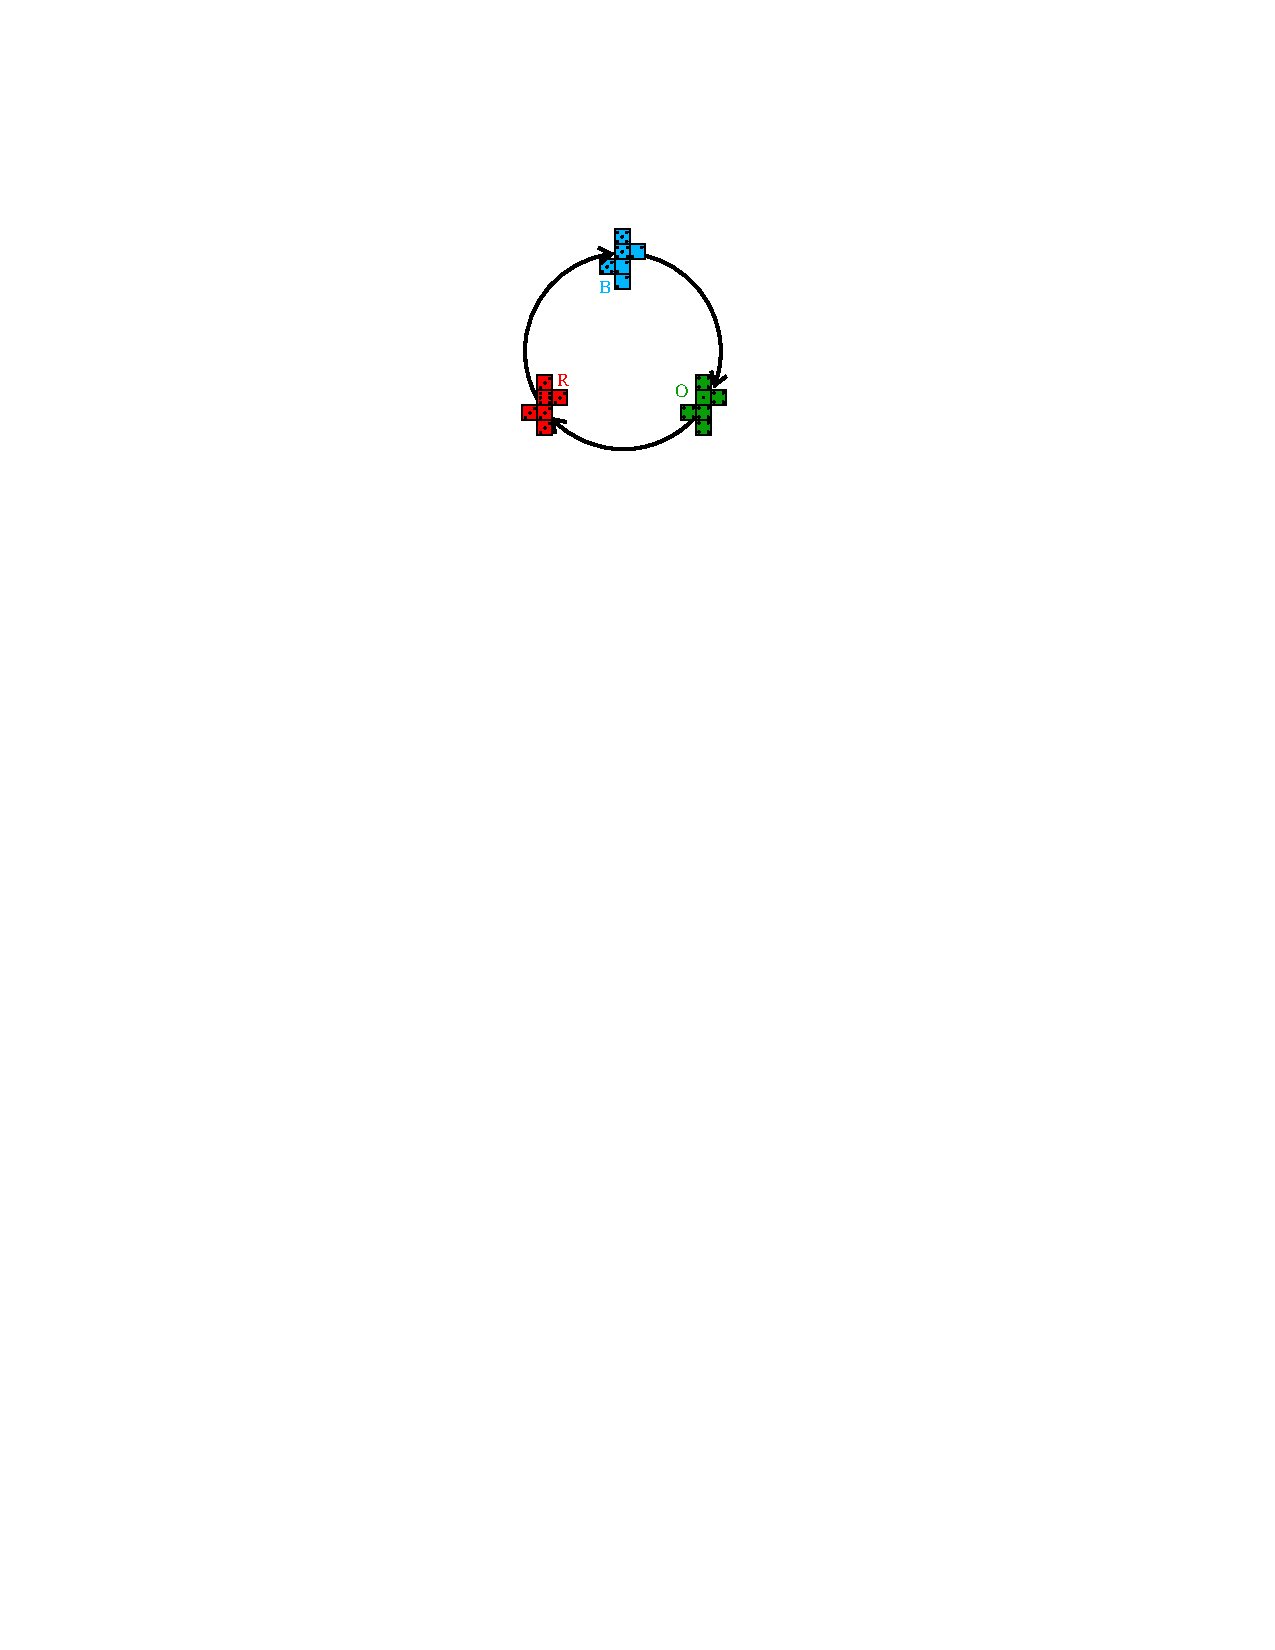
\includegraphics[scale =0.9]{4}
%		\caption{\small\textit{\color{}}}
		\vspace*{-15pt}
	\end{figure}
	Đây chính là mẹo của trò chơi, bởi miễn là bạn nhường đối thủ chọn trước, bạn sẽ luôn chọn được một con xúc xắc có xác suất thắng lớn hơn.
	\vskip 0.05cm
	\textbf{\color{quantoan}Thiệt đơn thiệt kép}
	\vskip 0.05cm
	Sau vài ván thua, đối thủ bắt đầu nghi ngờ, nhưng mọi chuyện vẫn chưa kết thúc. Sau khi giải thích chuỗi thắng bại vòng tròn của ba con xúc xắc, hãy thách bạn của bạn chơi một trò mới.
	\vskip 0.05cm
	Lần này, bạn chọn trước, và đối thủ sẽ có thể chọn một con xúc xắc có xác suất thắng lớn hơn. Nhưng cả số tiền cược lẫn số lần gieo đều tăng: mỗi người gieo con xúc xắc của mình hai lần, ai được tổng điểm lớn hơn thì thắng.
	\vskip 0.05cm
	Có lẽ với hai con xúc xắc thì đối thủ có xác suất thắng cũng gấp đôi? Nhưng không, thật kỳ diệu, với hai con xúc xắc, chuỗi thắng bại lại đảo chiều!
	\begin{figure}[H]
		\vspace*{-10pt}
		\centering
		\captionsetup{labelformat= empty, justification=centering}
		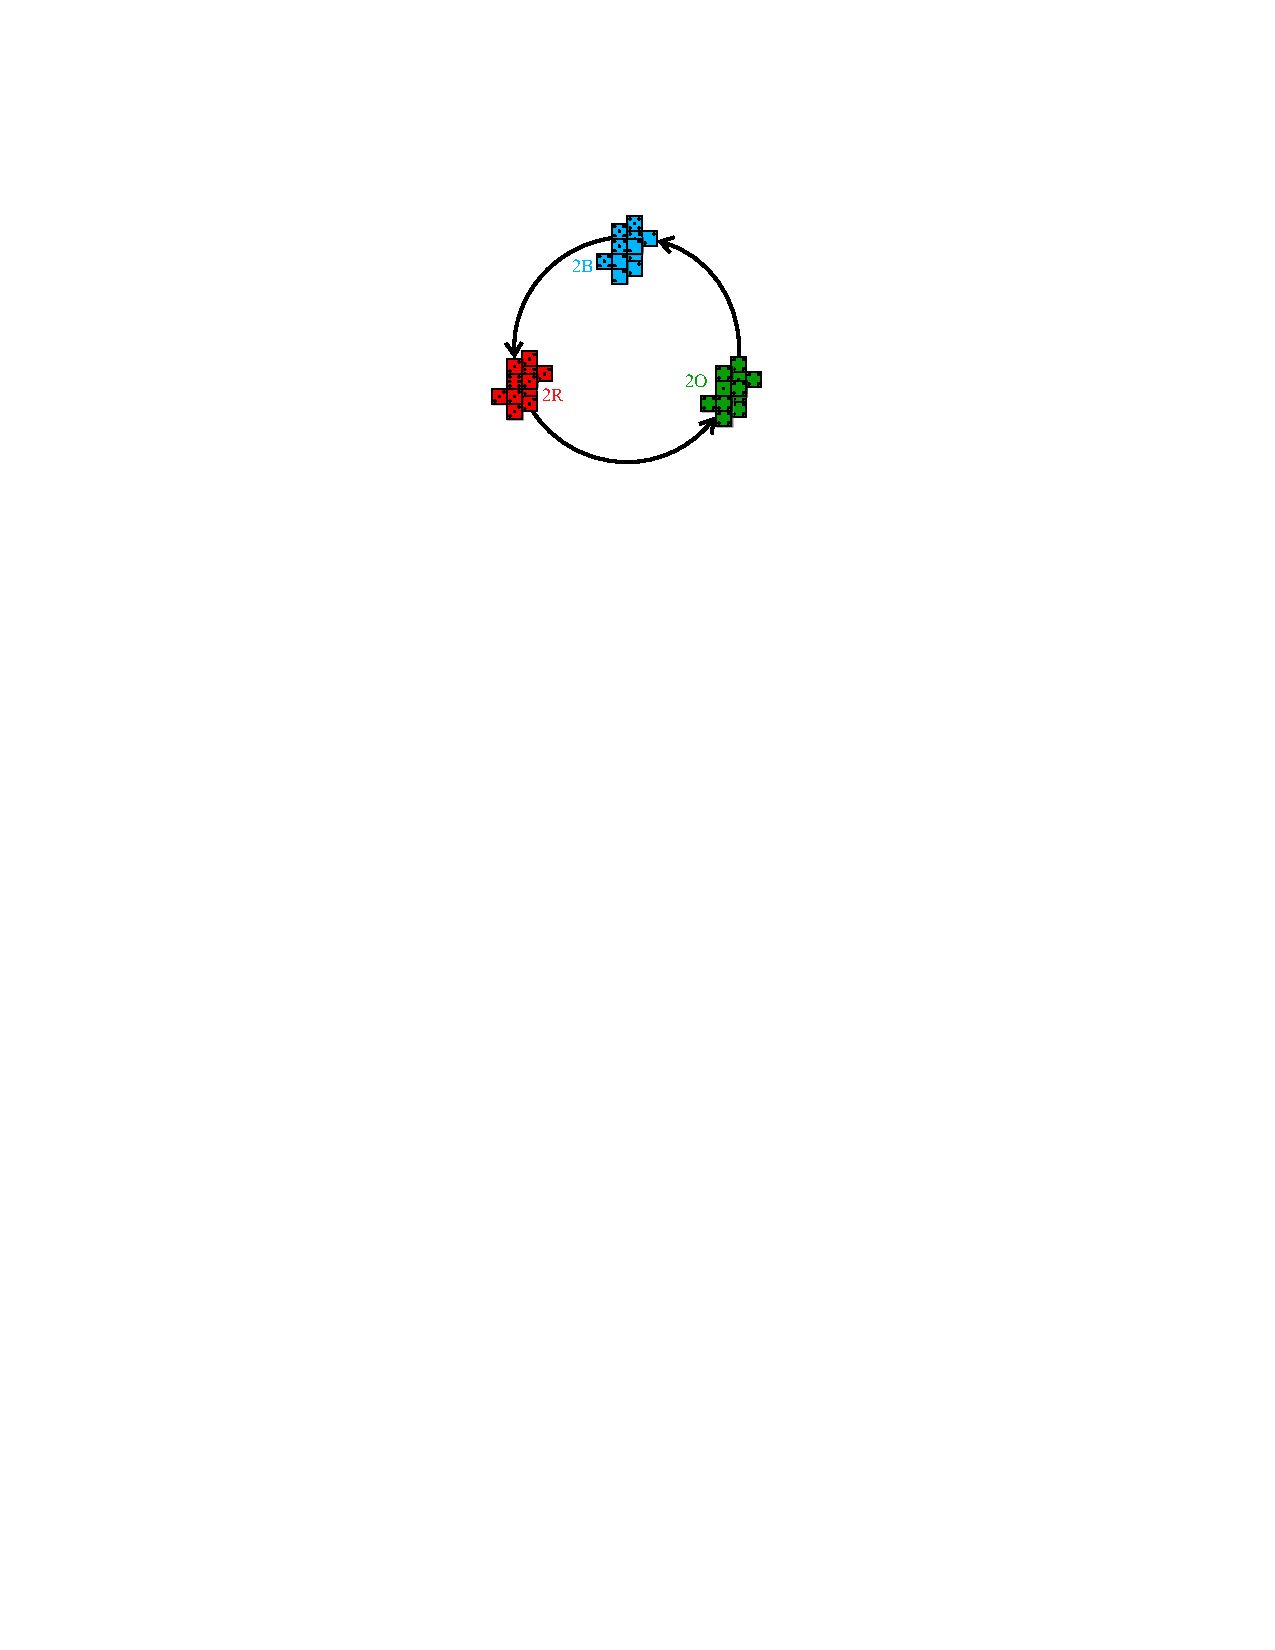
\includegraphics[scale =0.7]{5}
%		\caption{\small\textit{\color{}}}
		\vspace*{-15pt}
	\end{figure}
	Nói cách khác, vòng tròn thắng trở thành vòng tròn bại, nhờ đó bạn tiếp tục thắng trong trò chơi mới!
	\vskip 0.05cm
	\textbf{\color{quantoan}Bộ xúc xắc Efron}
	\vskip 0.05cm
	Bản chất nghịch lý của những con xúc xắc không bắc cầu được phát hiện vào năm $1959$, bởi hai nhà toán học Ba Lan Hugo Steinhaus và Stanislaw Trybuła [$3$].
	\vskip 0.05cm
	Tuy nhiên, tính chất đảo chiều đặc biệt không đúng cho mọi bộ xúc xắc không bắc cầu. Thí dụ, trong hình dưới đây là một bộ bốn con xúc xắc không bắc cầu được Martin Gardner giới thiệu vào năm $1970$ [$1$]. Chúng được tìm ra bởi nhà thống kê học người Mỹ Brad Efron.
	\begin{figure}[H]
		\vspace*{-5pt}
		\centering
		\captionsetup{labelformat= empty, justification=centering}
		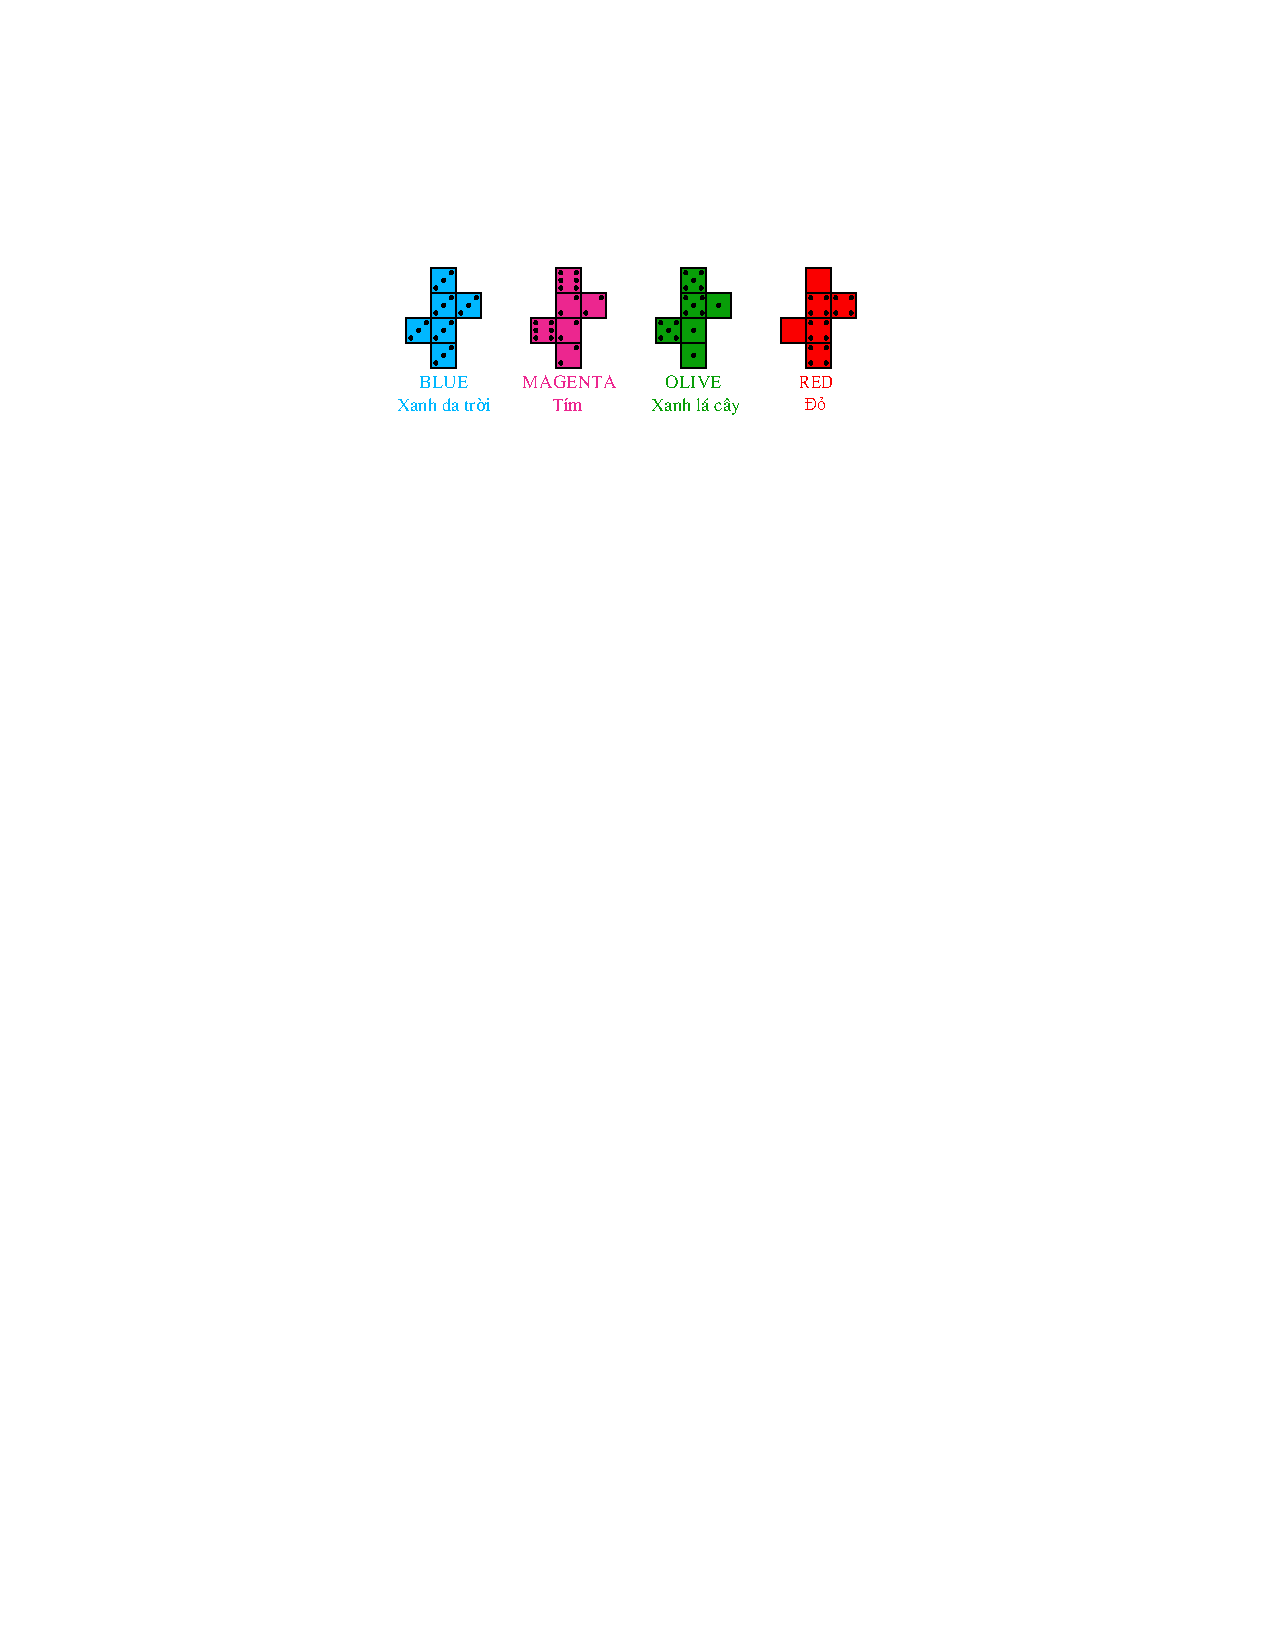
\includegraphics[width=1\linewidth]{6}
		\caption{\small\textit{\color{quantoan}Bộ xúc xắc Efron.}}
		\vspace*{-10pt}
	\end{figure}
	Ở đây, các con xúc xắc tạo thành một vòng tròn: Xanh da trời thắng Tím, Tím thắng Xanh lá cây, Xanh lá cây thắng Đỏ, và Đỏ thắng Xanh da trời, tất cả cùng với xác suất $2/3$.
	\begin{figure}[H]
		\vspace*{-10pt}
		\centering
		\captionsetup{labelformat= empty, justification=centering}
		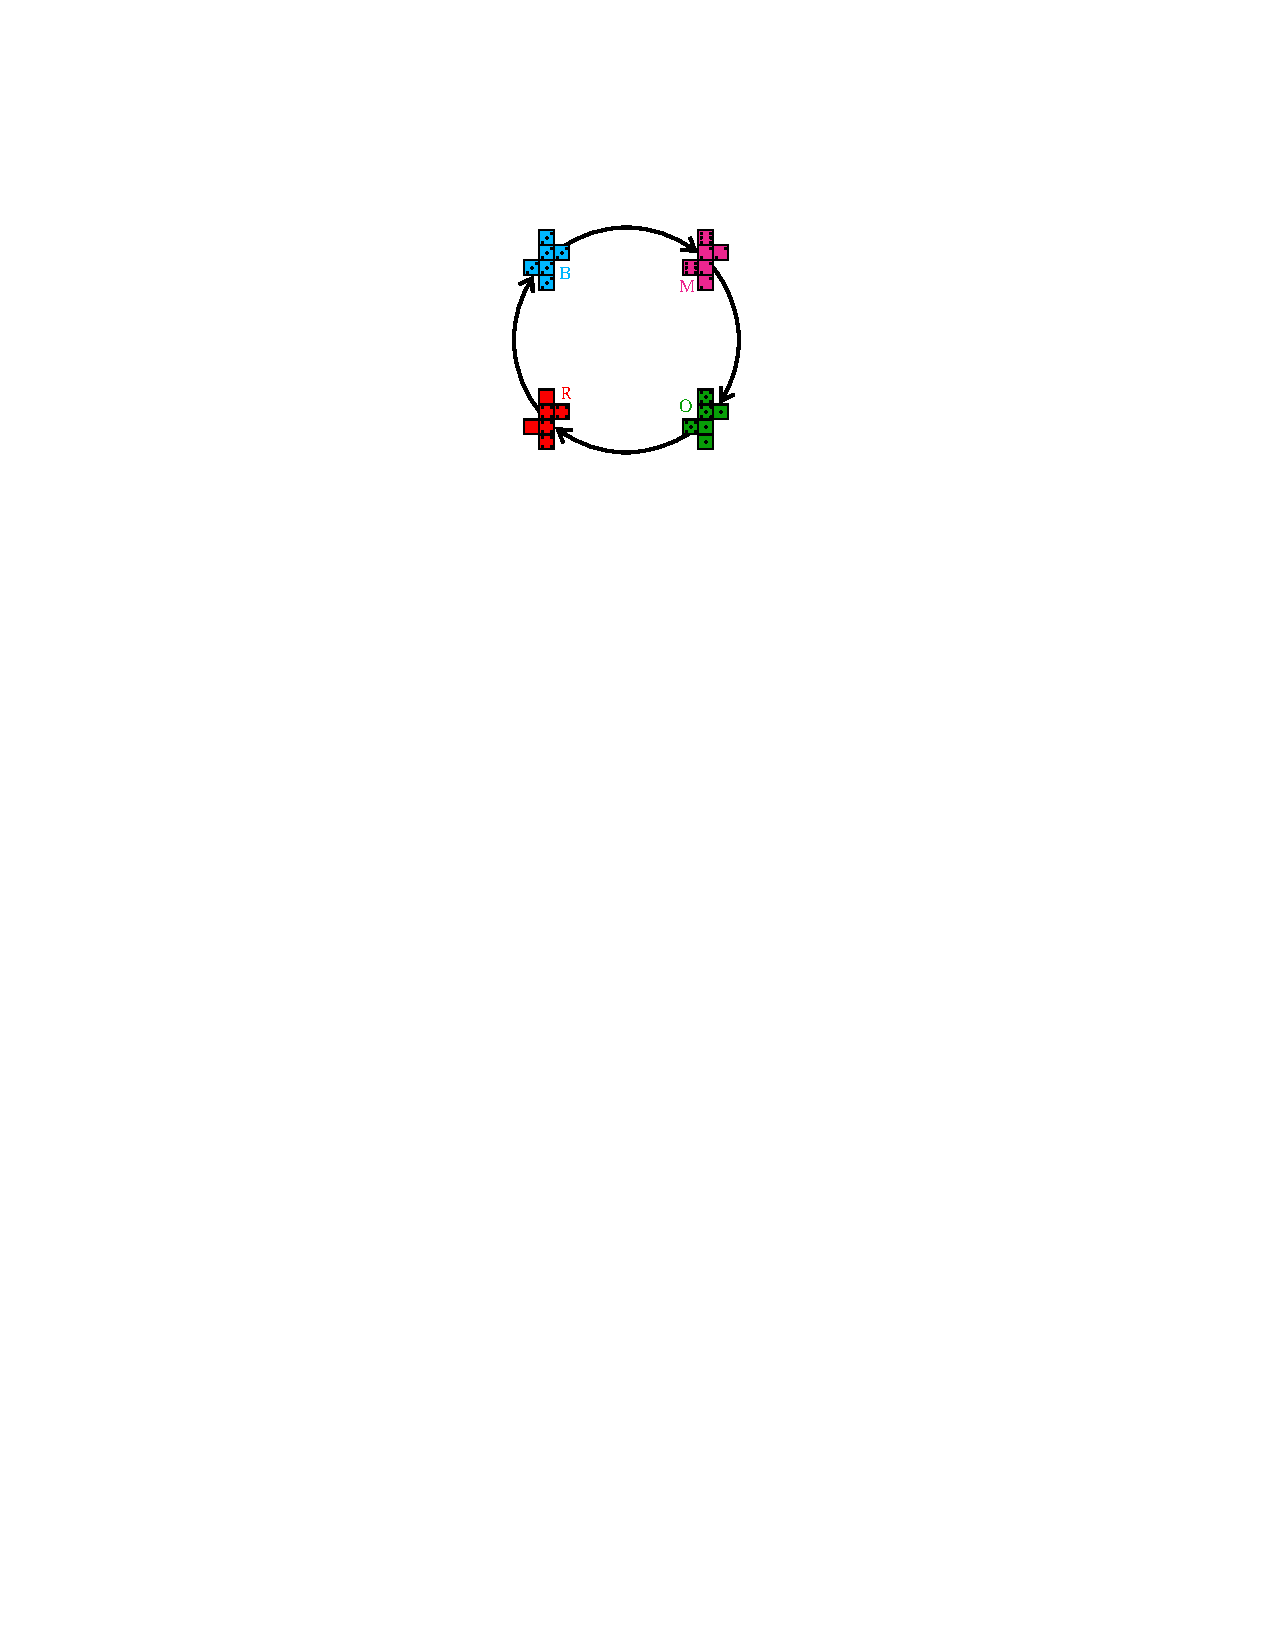
\includegraphics[scale =0.8]{7}
%		\caption{\small\textit{\color{}}}
		\vspace*{-10pt}
	\end{figure}
	Trong [$5$], Trybuła cũng chứng minh rằng luôn có thể tạo được một bộ xúc xắc không bắc cầu gồm $m$ con xúc xắc $n$ mặt, đồng thời chặn xác suất thắng nhỏ nhất của các con xúc xắc. Các xác suất thắng có thể đồng thời lớn hơn hoặc bằng, nhưng không thể đồng thời lớn hơn hẳn chặn này\footnote[3]{\color{quantoan}Nói cách khác, cận trên đúng của xác suất thắng nhỏ nhất -- ND.}.
	\vskip 0.05cm
	Trong trường hợp xúc xắc sáu mặt, bộ ba con xúc xắc đầu tiên đạt được chặn này. Với số mặt bất kỳ, giá trị chặn lớn nhất cho ba con xúc xắc là tỷ lệ vàng $\varphi = 0{,}618\dots$. Giá trị này tăng theo số con xúc xắc và hội tụ tới $3/4$.
	\vskip 0.05cm
	Bộ xúc xắc Efron đạt được giá trị chặn $2/3$ cho bốn con xúc xắc. Nhưng không may, chúng không có tính chất đảo chiều khi gấp đôi số lần gieo. Một số quan hệ thắng bại đổi chiều, số khác thì không.
	\vskip 0.05cm
	Nghe đồn rằng tỷ phú Mỹ Warren Buffet rất thích những con xúc xắc không bắc cầu. Khi ông thách người bạn Bill Gates chơi một trò chơi với bộ xúc xắc Efron, Bill Gates đã nghi hoặc và đòi Warren Buffet chọn trước. Có lẽ nếu Warren Buffet dùng một bộ xúc xắc có tính chất đảo chiều, ông đã có thể thắng Bill Gates -- ông chỉ cần tuyên bố gieo một lần hay gieo hai lần sau khi cả hai đã chọn xong xúc xắc.
	\vskip 0.05cm
	\textbf{\color{quantoan}Trò chơi ba người}
	\vskip 0.05cm
	Tôi muốn biết liệu có thể mở rộng ý tưởng xúc xắc không bắc cầu để tạo ra một trò chơi ba người hay không, nghĩa là có hay không một bộ xúc xắc sao cho sau khi hai người bạn mỗi người đã chọn một con xúc xắc, bạn có thể chọn một con xúc xắc thắng cả hai con xúc xắc của họ!
	\vskip 0.05cm
	Hóa ra là có thể. M. Oskar van Deventer, nhà thiết kế trò chơi người Hà Lan, đã tìm ra một bộ bảy con xúc xắc với các giá trị từ $1$ đến $21$. Trong bộ xúc xắc này, hai đối thủ có thể chọn mỗi người một con xúc xắc bất kỳ, và luôn có một con xúc xắc thứ ba thắng được cả hai. Các xác suất thắng đối xứng một cách đẹp đẽ: mỗi mũi tên trong sơ đồ dưới đây đều biểu diễn một xác suất thắng bằng $5/9$.
	\vskip 0.05cm
	Điều này có nghĩa là bạn có thể đồng thời đấu với hai người. Tuy nhiên, vẫn không dễ thắng được cả hai cùng một lúc. Xác suất để thắng được cả hai cùng một lúc chỉ khoảng $39\%$.
	\begin{figure}[H]
		\vspace*{-10pt}
		\centering
		\captionsetup{labelformat= empty, justification=centering}
		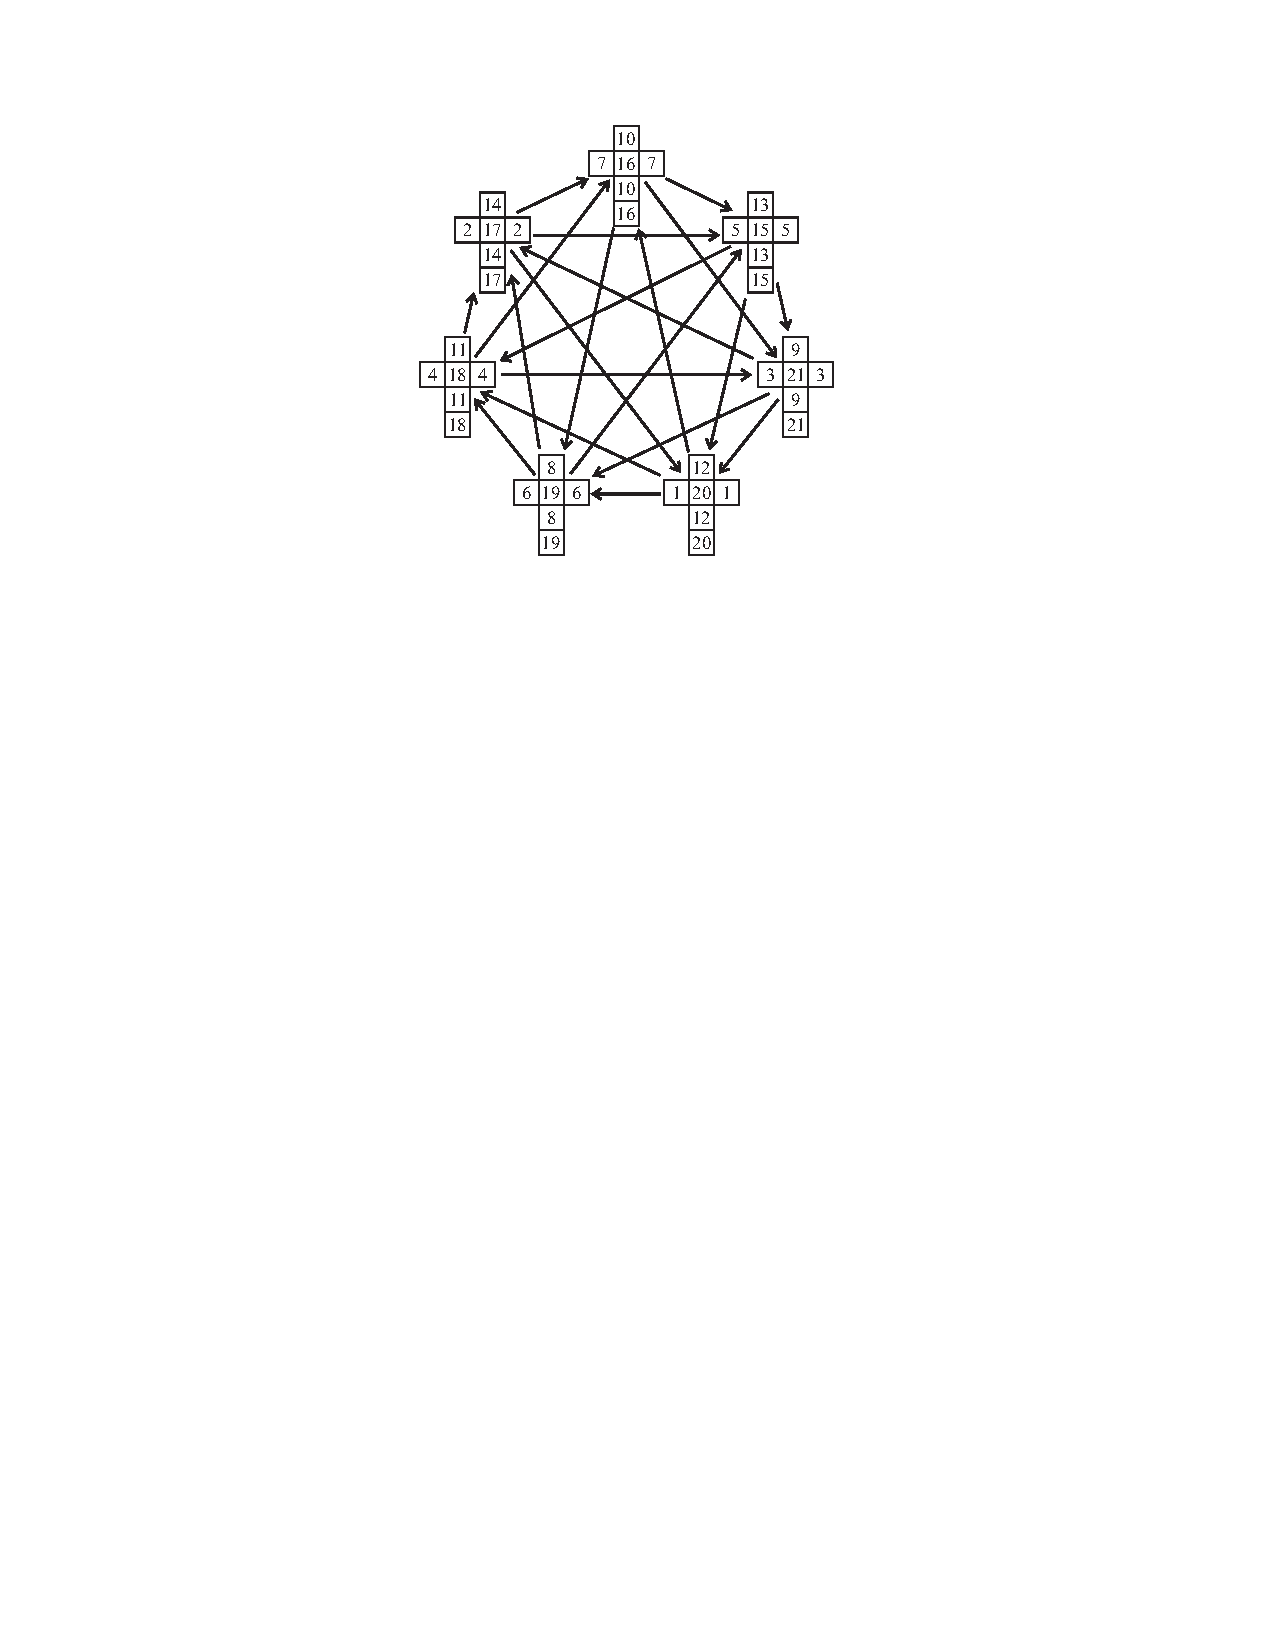
\includegraphics[scale =0.6]{8}
		\caption{\small\textit{\color{quantoan}Bộ xúc xắc Oskar.}}
		\vspace*{-10pt}
	\end{figure}
	Bộ bảy con xúc xắc này tạo thành một đồ thị có hướng đầy đủ. Một cách tương tự, trò chơi bốn người sẽ cần $19$ con xúc xắc. Chúng ta chưa biết liệu có tồn tại một bộ xúc xắc như vậy hay không.
	\vskip 0.05cm
	Tuy nhiên, tôi bắt đầu suy nghĩ xem liệu có thể tận dụng tính chất đảo chiều của một số con xúc xắc không bắc cầu để thiết kế một trò chơi ba người hơi khác đi một chút, với ít hơn bảy con xúc xắc.
	\vskip 0.1cm
	\textbf{\color{quantoan}Bộ xúc xắc Grime}
	\vskip 0.1cm
	Ý tưởng về trò chơi ba người của tôi sử dụng năm con xúc xắc với hai chuỗi thắng bại vòng tròn. Khi gấp đôi số lần gieo, một chuỗi sẽ giữ nguyên, còn chuỗi kia đảo chiều. Khi đó, bằng cách chọn gieo một lần hay hai lần, bạn sẽ có thể đấu với hai người cùng một lúc, bất kể họ chọn như thế nào.
	\begin{figure}[H]
		\vspace*{-10pt}
		\centering
		\captionsetup{labelformat= empty, justification=centering}
		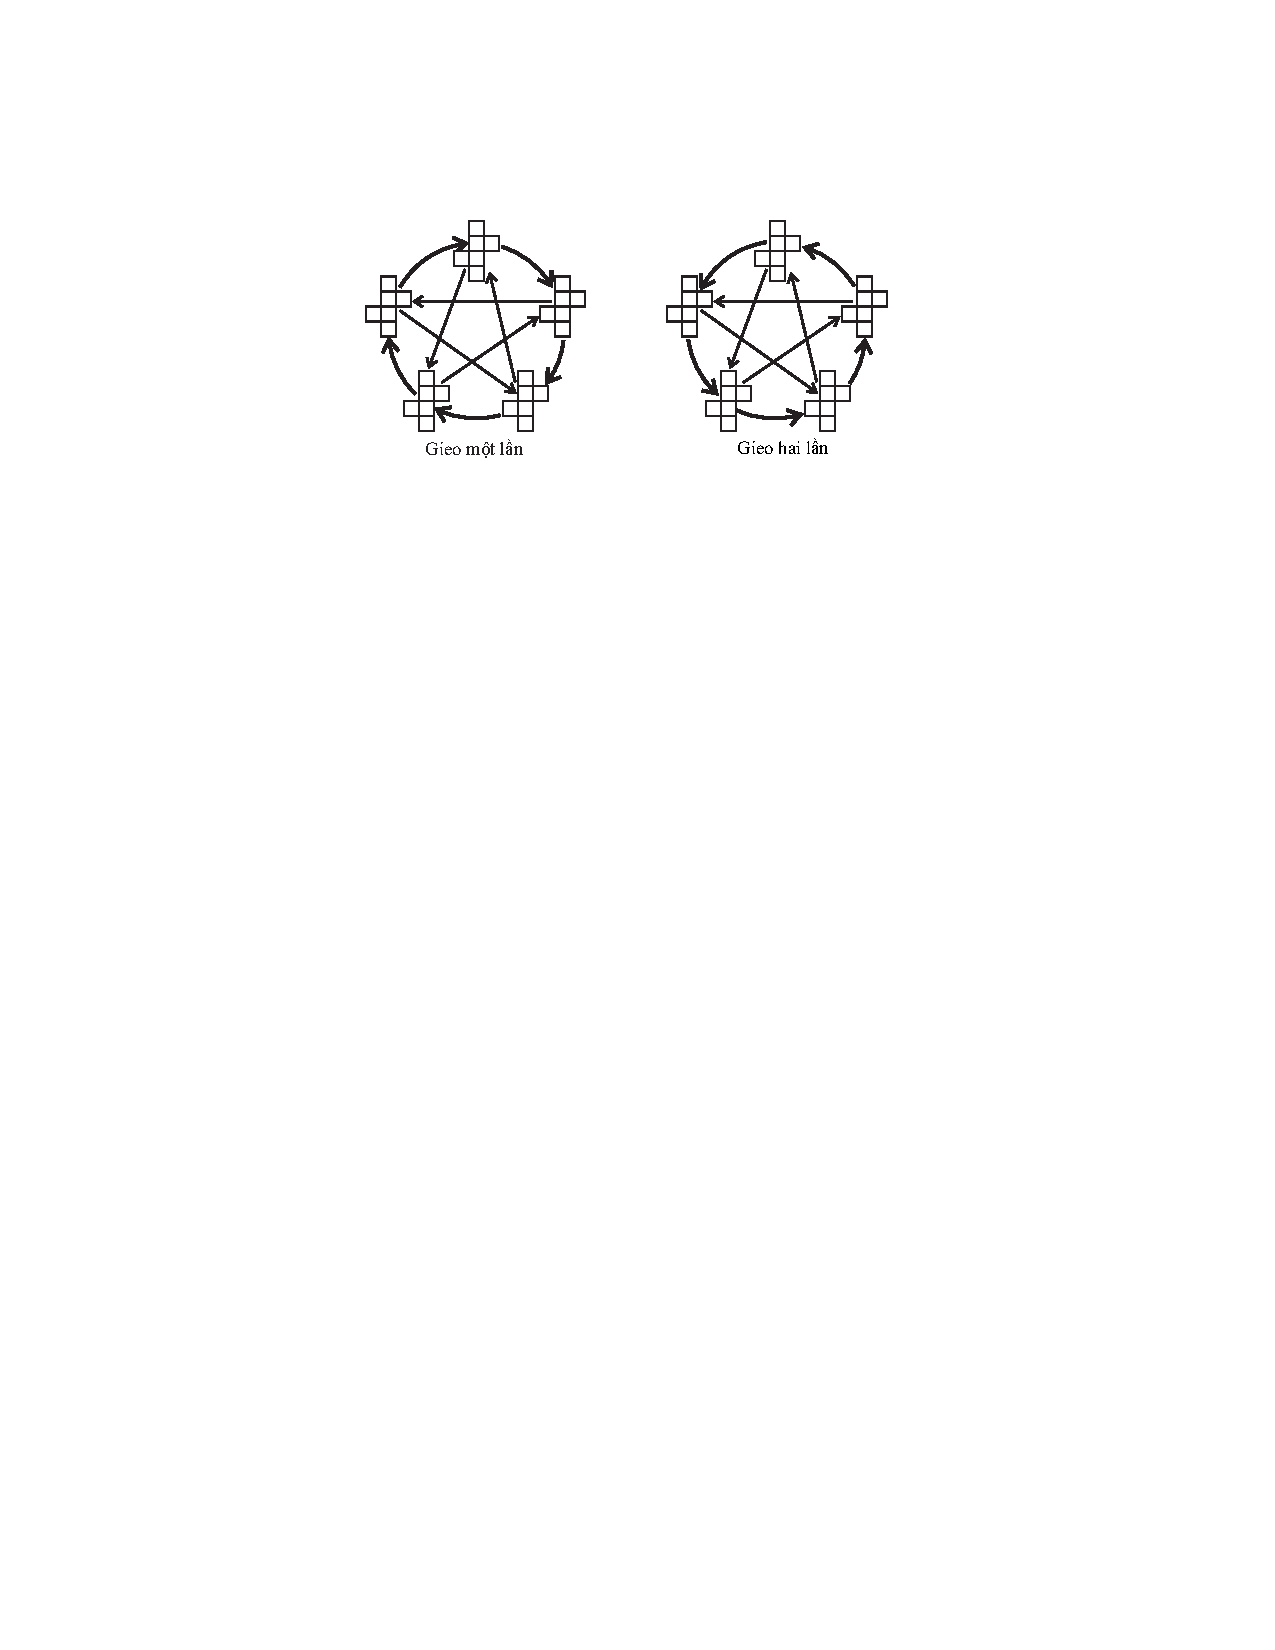
\includegraphics[width = 1\linewidth]{9}
%		\caption{\small\textit{\color{}}}
		\vspace*{-25pt}
	\end{figure}
	Sau một hồi mò mẫm, tôi tìm được bộ năm con xúc xắc không bắc cầu dưới đây.
	\begin{figure}[H]
%		\vspace*{5pt}
		\centering
		\captionsetup{labelformat= empty, justification=centering}
		
\includegraphics[width = 1\linewidth]{10}
		\caption{\small\textit{\color{quantoan}Bộ xúc xắc Grime.}}
		\vspace*{-15pt}
	\end{figure}
	Có vẻ như đây là bộ tốt nhất tôi có thể tìm được. Tôi đã từng viết về chúng, và chúng được đặt tên là bộ xúc xắc Grime.
	\vskip 0.05cm
	Với một lần gieo, ta có hai chuỗi thắng bại như sau.
	\vskip 0.05cm
	Tất cả các xác suất thắng đều bằng $5/9$, và xác suất thắng trung bình là $63\%$ (việc kiểm tra các tính toán này được dành cho người đọc). Để ý rằng một chuỗi tuân theo thứ tự bảng chữ cái, còn chuỗi kia được sắp xếp theo số chữ cái [của từ tiếng Anh].
	\begin{figure}[H]
		\vspace*{-5pt}
		\centering
		\captionsetup{labelformat= empty, justification=centering}
		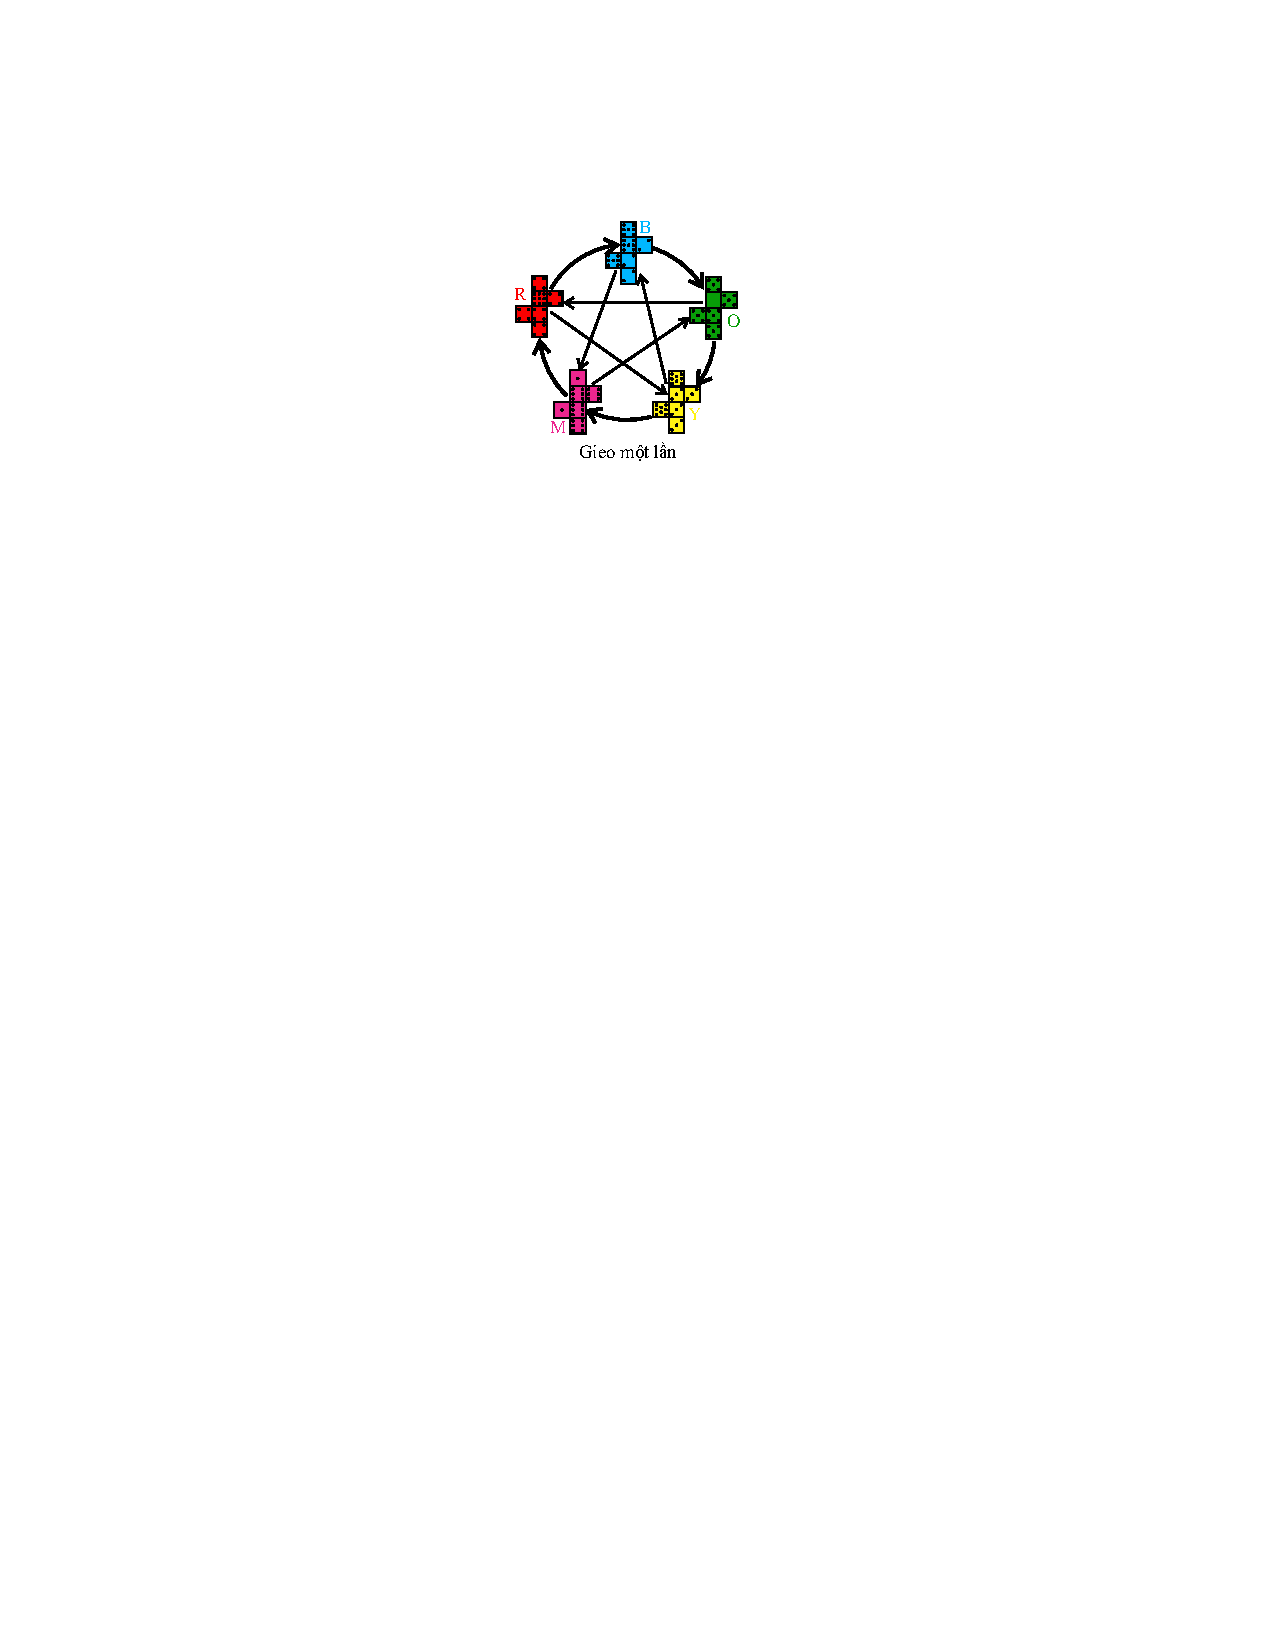
\includegraphics[scale =1]{11}
		%		\caption{\small\textit{\color{}}}
		\vspace*{-10pt}
	\end{figure}
	Bạn cũng có thể tìm thấy những bộ xúc xắc không bắc cầu nhỏ hơn. Chẳng hạn, ba con xúc xắc Đỏ, Xanh da trời, Xanh lá cây chính là bộ ba được mô tả ở đầu bài viết, với cùng các xác suất thắng và tính chất đảo chiều.
	\vskip 0.05cm
	Với hai lần gieo, ta có các chuỗi thắng bại như sau.
	\begin{figure}[H]
		\vspace*{-5pt}
		\centering
		\captionsetup{labelformat= empty, justification=centering}
		
\includegraphics[scale =1]{12}
%		\caption{\small\textit{\color{}}}
		\vspace*{-10pt}
	\end{figure}
	Khi gấp đôi số lần gieo, vòng tròn bên ngoài đảo chiều còn ngôi sao bên trong giữ nguyên, nhưng có một ngoại lệ do tính chất đảo chiều của ba con xúc xắc Đỏ, Xanh da trời, Xanh lá cây.
	\vskip 0.05cm
	Tuy nhiên, xác suất của ngoại lệ này rất gần với $50\%$ (chính xác là $625/1296$). Trong khi đó, trung bình của tất cả các xác suất thắng còn lại là $62\%$ (cao hơn hẳn so với bộ xúc xắc Oskar), do đó trong thực tế trò chơi ba người vẫn hiệu quả.
	\vskip 0.05cm
	Khá là thú vị khi bộ năm con xúc xắc này chứa ba con xúc xắc có tính chất đảo chiều. Tuy nhiên, thú thực là chỗ ngoại lệ vẫn khiến tôi lăn tăn. Tôi muốn biết có tìm được bộ năm con xúc xắc không bắc cầu thỏa mãn các tính chất cần tìm, không có ngoại lệ, hay không, hay đây là bộ tốt nhất có thể.
	\vskip 0.1cm
	\textbf{\color{quantoan}Đi tìm một bộ xúc xắc Grime mới}
	\vskip 0.1cm
	Tôi tìm đến sự trợ giúp của máy tính và sự trợ giúp vô giá của người bạn Brian Pollock, để tìm các bộ năm con xúc xắc không bắc cầu. Việc xem xét tất cả các bộ năm con xúc xắc cùng với các chuỗi thắng bại của chúng là một thách thức tính toán khổng lồ, vì vậy chúng tôi tạo ra một phép thử.
	\vskip 0.05cm
	Ba con xúc xắc tạo ra một sơ đồ hoặc với ba mũi tên cùng chiều, mà ta gọi là chuỗi không bắc cầu, hoặc với chỉ hai mũi tên cùng chiều, mà ta gọi là chuỗi bắc cầu.
	\begin{figure}[H]
		\vspace*{-10pt}
		\centering
		\captionsetup{labelformat= empty, justification=centering}
		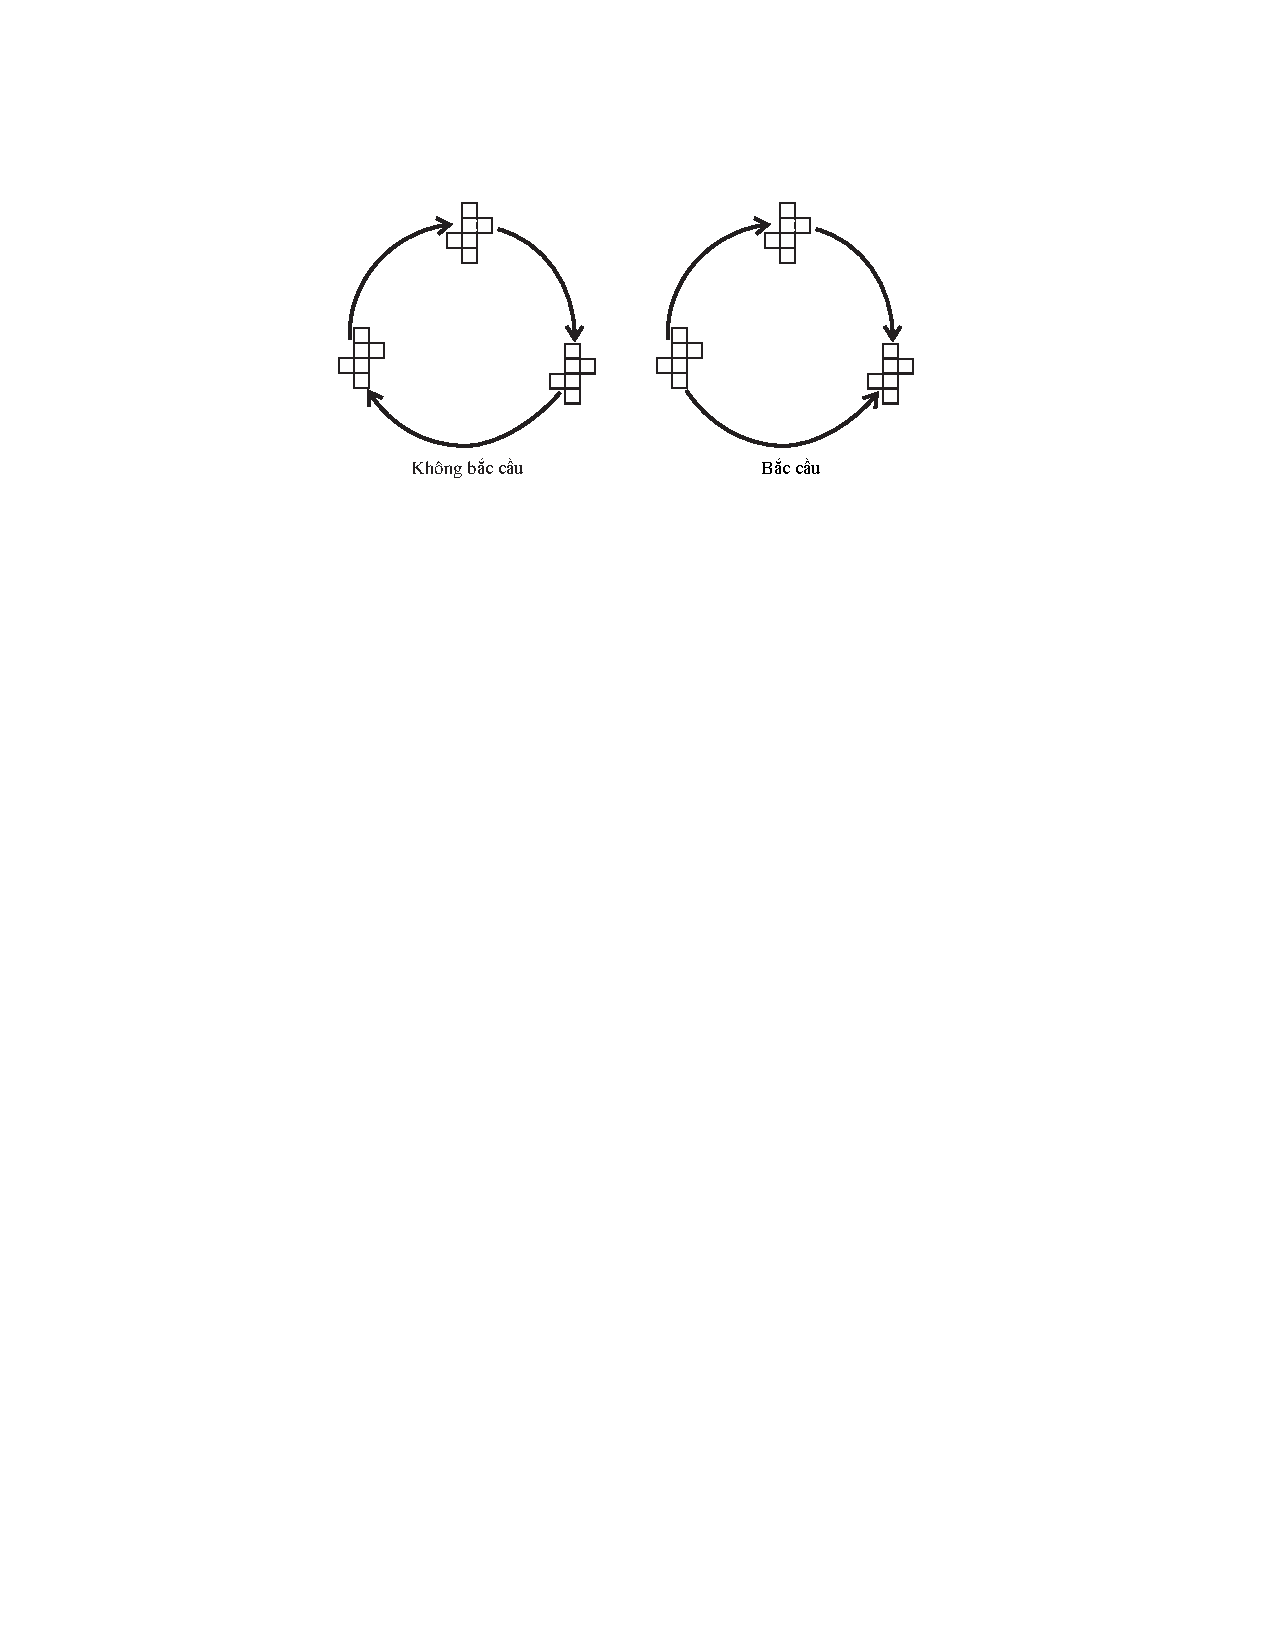
\includegraphics[width=1\linewidth]{13}
%		\caption{\small\textit{\color{}}}
		\vspace*{-25pt}
	\end{figure}
	Chúng tôi muốn tạo ra một bộ năm con xúc xắc không bắc cầu với hai chuỗi không bắc cầu, sao cho khi nhân đôi số lần gieo, một chuỗi giữ nguyên còn một chuỗi đảo chiều.
	\vskip 0.05cm
	Điều này có nghĩa là với mọi bộ ba trong năm con xúc xắc, nếu chúng tạo thành một chuỗi không bắc cầu với một lần gieo, thì với hai lần gieo chúng sẽ tạo thành một chuỗi bắc cầu. Nếu một chuỗi giữ nguyên tính bắc cầu hoặc không bắc cầu khi gấp đôi số lần gieo, ta nói bộ ba con xúc xắc đó không qua được phép thử.
	\vskip 0.05cm
	Mỗi bộ năm con xúc xắc có $10$ bộ ba. Mọi bộ ba đều cần qua được phép thử. Hơn nữa, nếu mọi bộ ba qua được phép thử thì chúng ta đã tìm được một bộ năm con xúc xắc thỏa mãn.
	\vskip 0.05cm
	Phép thử này cho phép chúng tôi tốn ít tính toán hơn để loại các bộ không thỏa mãn.
	\vskip 0.05cm
	Ban đầu, chúng tôi chỉ xét các con xúc xắc có các giá trị từ $0$ đến $9$. Các bộ có kết quả hòa thì không hay lắm. Nhưng sau khi loại các bộ có kết quả hòa, không có bộ năm con xúc xắc nào qua được phép thử.
	\vskip 0.05cm
	Chỉ có một số ít bộ bốn con xúc xắc qua được phép thử, chúng chính là bộ xúc xắc Grime bỏ đi một con. Điều này chứng tỏ bộ xúc xắc Grime quả đúng là bộ tốt nhất với các giá trị từ $0$ đến $9$ và không có hòa.
	\vskip 0.1cm
	\textbf{\color{quantoan}Với giá trị lớn hơn}
	\vskip 0.1cm
	Một cách tự nhiên, bước tiếp theo là thử tìm những con xúc xắc với giá trị lớn hơn. Vẫn với tiêu chuẩn không hòa, kết quả đầu tiên sử dụng các giá trị từ $0$ đến $13$.
	\begin{table}[H]
		\vspace*{-10pt}
		\centering
		\renewcommand{\arraystretch}{1.1}
		\begin{tabular}{|c|c|c|c|c|c|c|}
			\hline
			$A$ &$4$& $4$& $4$& $4$& $4$& $9$\\
			\hline
			$B$ &$2$& $2$& $2$& $7$& $7$& $12$\\
			\hline
			$C$ &$0$& $5$& $5$& $5$& $5$& $10$\\
			\hline
			$D$ &$3$& $3$& $3$& $3$& $8$& $13$\\
			\hline
			$E$ &$1$& $1$& $6$& $6$& $6$& $11$\\
			\hline
		\end{tabular}
		\vspace*{-10pt}
	\end{table}
	Có hai bộ như vậy sử dụng các giá trị từ $0$ đến $13$, bộ thứ hai chỉ khác bộ trên một chút xíu. Chúng cũng là những bộ năm duy nhất với các giá trị liên tiếp.
	\vskip 0.05cm
	Tôi rất sung sướng với kết quả này, nhưng xác suất thắng trung bình chỉ là $59\%$, thấp hơn bộ xúc xắc Grime. Vì vậy, chúng tôi tiếp tục đi tìm một bộ với xác suất thắng lớn hơn.
	\vskip 0.05cm
	Xác suất thắng tăng một cách chậm chạp theo các giá trị trên mặt xúc xắc. Dưới đây là một trong những bộ mạnh nhất, sử dụng các giá trị từ $0$ đến $17$.
	\begin{table}[H]
		\vspace*{5pt}
		\centering
		\renewcommand{\arraystretch}{1.21}
		\begin{tabular}{|c|c|c|c|c|c|c|}
			\hline
			$A$ &$4$& $4$& $8$& $8$& $8$& $17$\\
			\hline
			$B$ &$2$& $2$& $2$& $15$& $15$& $15$\\
			\hline
			$C$ &$0$& $9$& $9$& $9$& $9$& $9$\\
			\hline
			$D$ &$3$& $3$& $3$& $3$& $16$& $16$\\
			\hline
			$E$ &$1$& $1$& $10$& $10$& $10$& $10$\\
			\hline
		\end{tabular}
		\vspace*{-10pt}
	\end{table}
	Đến lúc này, tăng giá trị không cải thiện xác suất thắng nữa. Vì các giá trị không còn là các số liên tiếp, một số giá trị có thể xê dịch trong các khoảng mà không ảnh hưởng đến xác suất thắng, nghĩa là bộ này có thể lặp lại dưới những dạng hơi khác đi một chút. Việc tìm kiếm những bộ tốt hơn đã chững lại.
	\vskip 0.05cm
	Vì lý do thẩm mỹ, tôi quyết định bớt đi $8$ ở mỗi mặt, kết quả nhận được là một bộ xúc xắc Grime mới, với các giá trị từ $-8$ đến $9$:
	\begin{figure}[H]
		\vspace*{-10pt}
		\centering
		\captionsetup{labelformat= empty, justification=centering}
		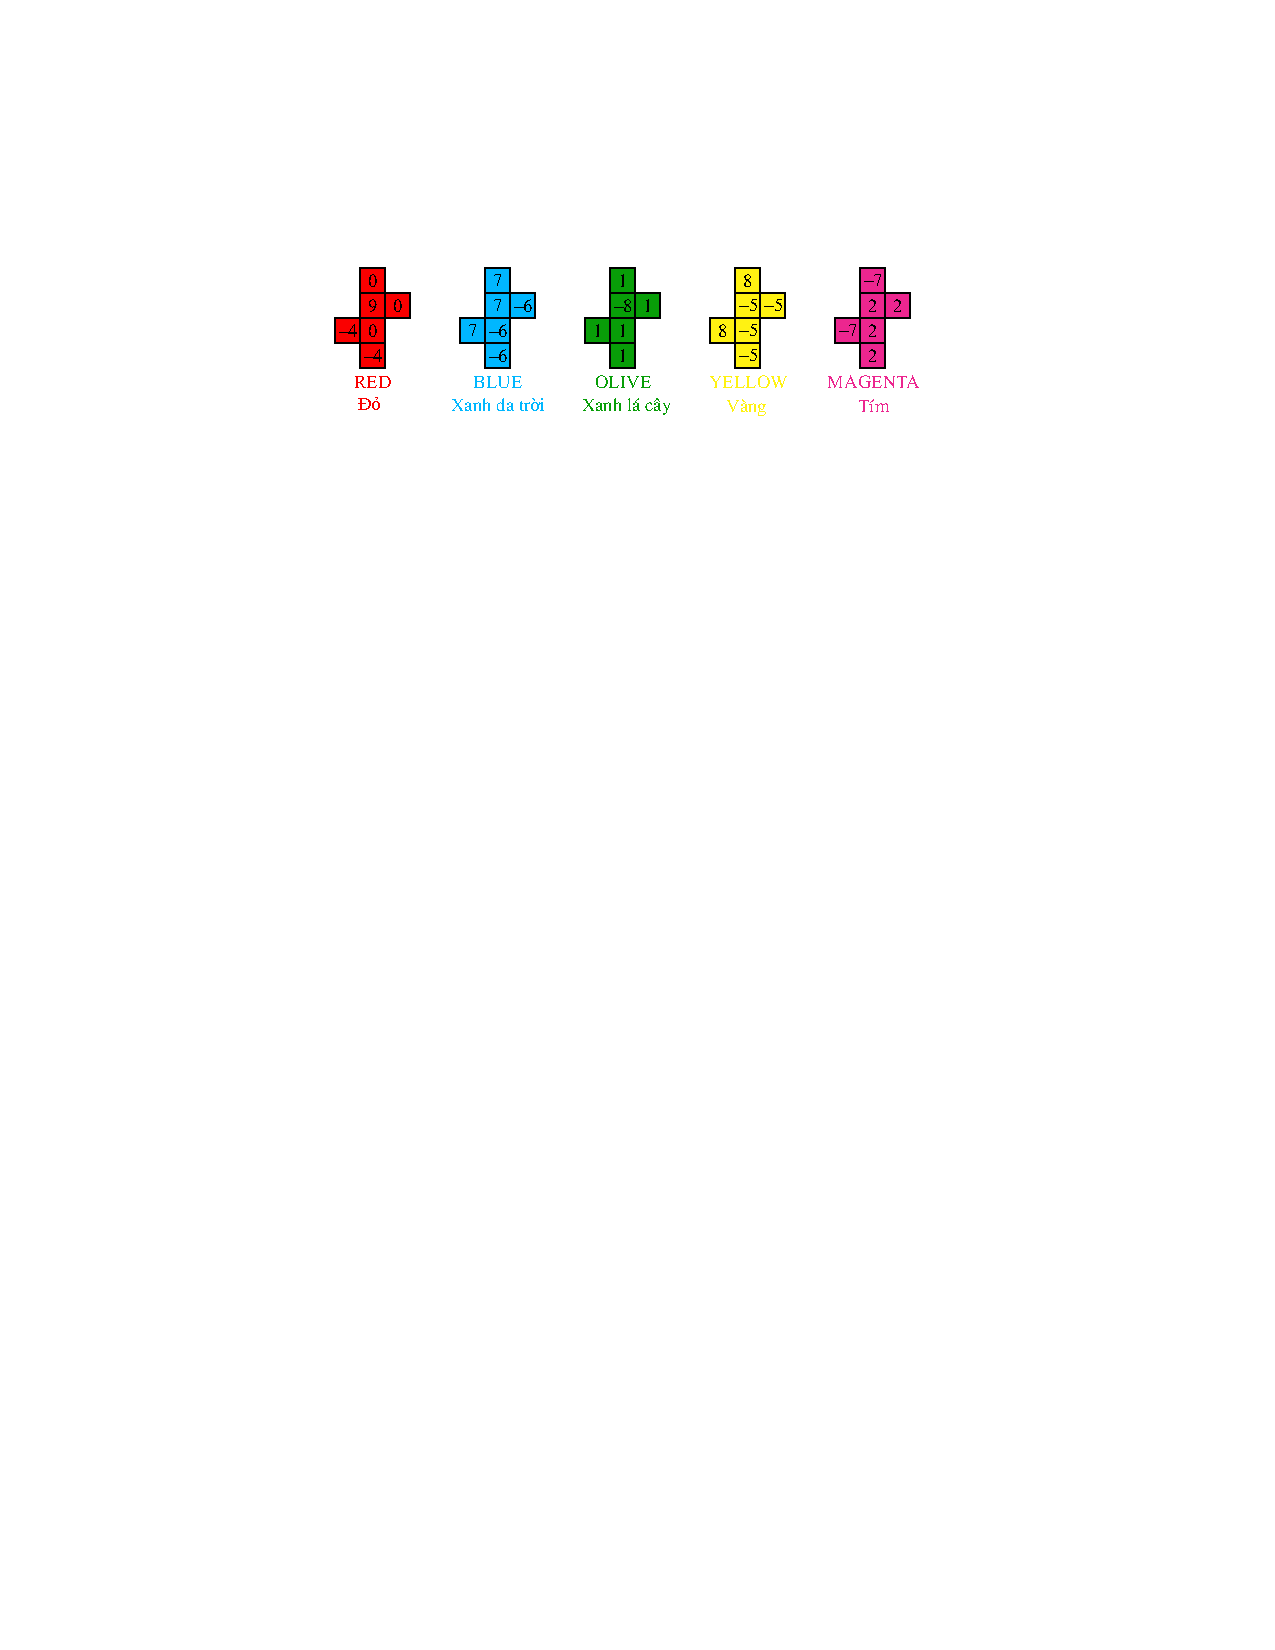
\includegraphics[width=1\linewidth]{14}
		\caption{\small\textit{\color{quantoan}Bộ xúc xắc Grime mới.}}
		\vspace*{-15pt}
	\end{figure}
	Cũng như bộ xúc xắc Grime gốc, bộ này tạo ra hai chuỗi không bắc cầu, một theo thứ tự bảng chữ cái, một theo số chữ cái. Khi gieo hai lần, chuỗi thứ nhất giữ nguyên, trong khi chuỗi thứ hai đảo chiều.
	\begin{figure}[H]
		\vspace*{-10pt}
		\centering
		\captionsetup{labelformat= empty, justification=centering}
		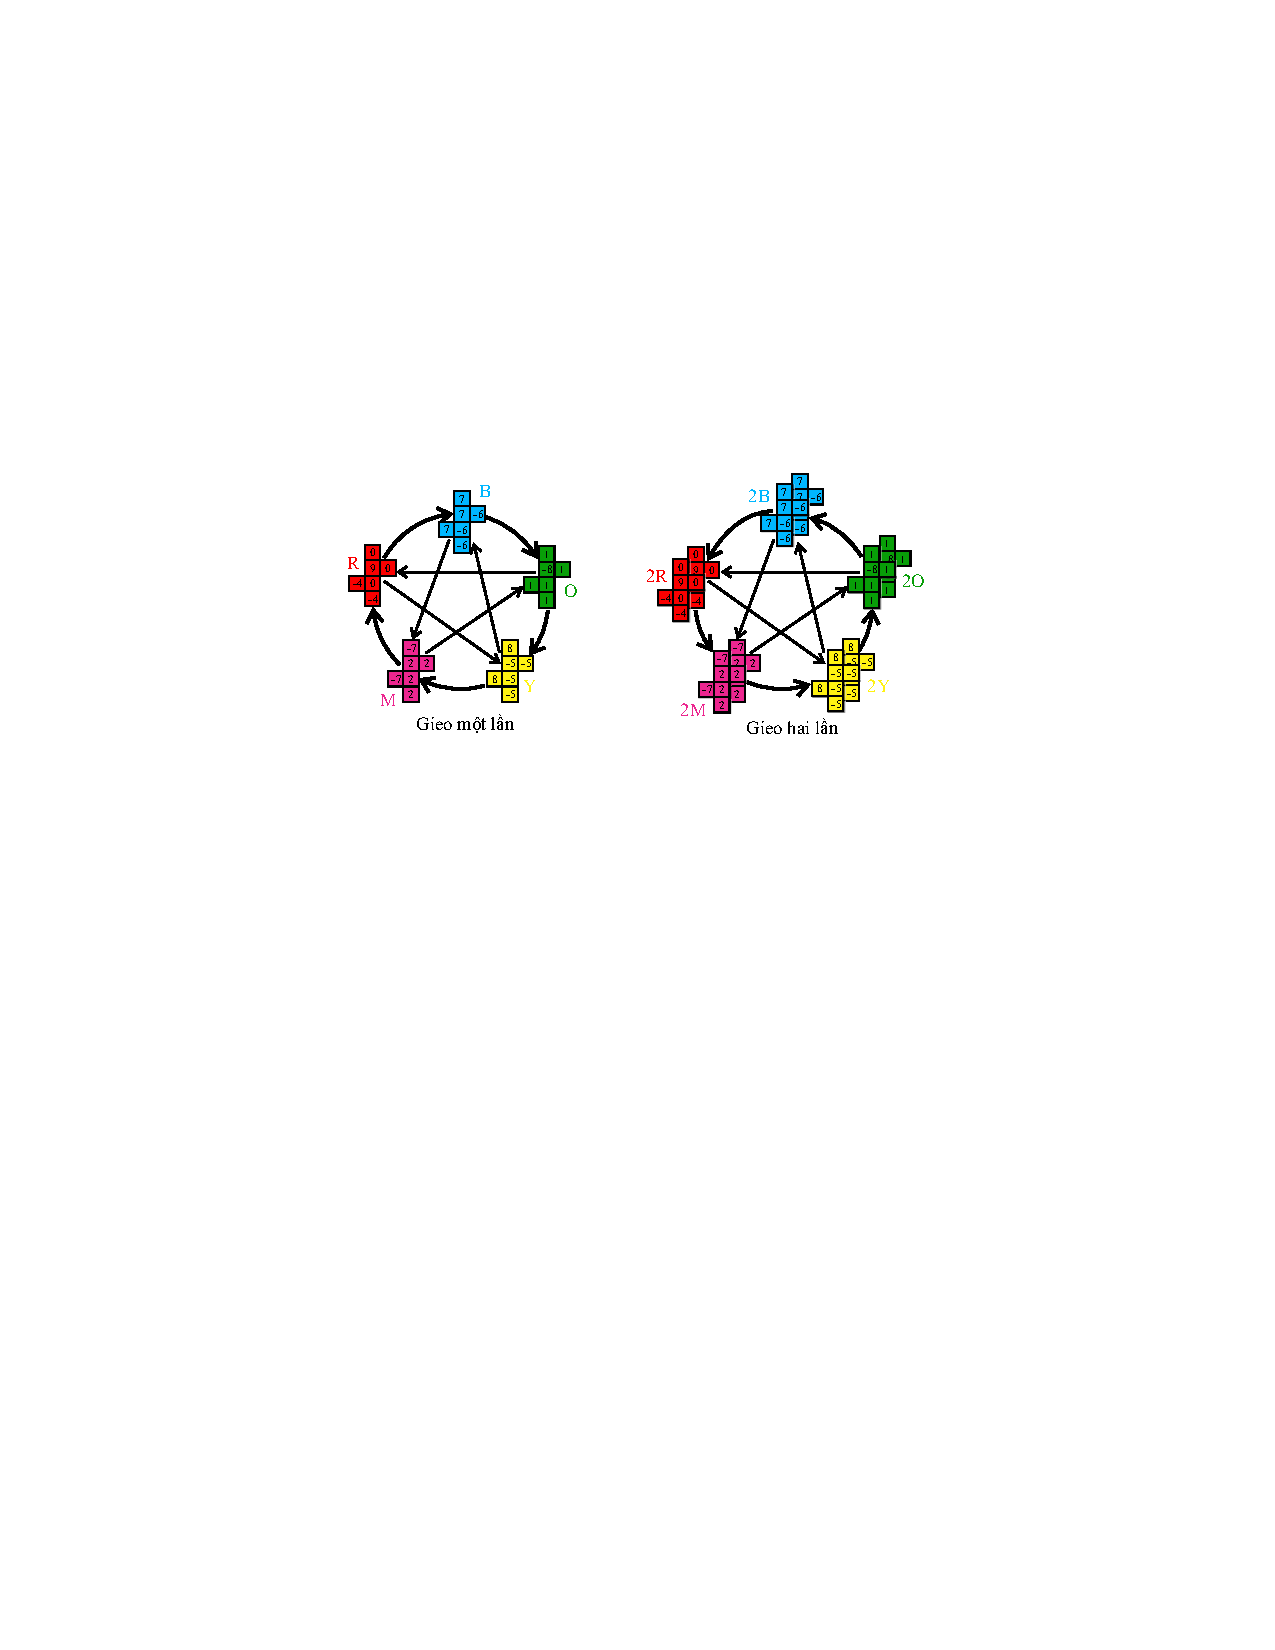
\includegraphics[width=1\linewidth]{15}
%		\caption{\small\textit{\color{}}}
		\vspace*{-20pt}
	\end{figure}
	Trong trò chơi một lần gieo, bộ Grime mới có xác suất thắng giống hệt bộ Grime gốc. Khi gieo hai lần, bộ mới nói chung yếu hơn, với xác suất thắng trung bình $60{,}4\%$, kém $0{,}7\%$ so với bộ gốc. Tuy nhiên, điểm quan trọng là mọi xác suất thắng đều lớn hơn $50\%$, từ đó cho phép tạo ra một trò chơi ba người thực sự như sau.
	\vskip 0.05cm
	Mời hai người mỗi người chọn một con xúc xắc, nhưng không nói trước sẽ gieo một lần hay hai lần. Bất kể họ chọn thế nào, bạn cũng sẽ chọn được một con xúc xắc thắng được cả hai. Nếu họ chọn hai con xúc xắc liền nhau theo thứ tự bảng chữ cái, hãy chơi phiên bản một lần gieo. Nếu họ chọn hai con xúc xắc liền nhau theo số chữ cái, hãy chơi phiên bản hai lần gieo. 
	\vskip 0.1cm
	\textbf{\color{quantoan}Một trò cá cược}
	\vskip 0.1cm
	Liệu chúng ta có thể kỳ vọng thắng cả hai người? Chúng ta dĩ nhiên đã cải thiện cơ hội, với xác suất trung bình để thắng cả hai người vào khoảng $44\%$, tăng $5\%$ so với bộ xúc xắc Oskar. Nhưng như vậy, với xác suất thắng cả hai dưới $50\%$, chúng ta làm thế nào để thắng? Hãy xét trò chơi sau đây.
	\vskip 0.1cm
	Thách hai người bạn chơi một trò xúc xắc, trong đó bạn đồng thời đấu với cả hai. Nếu thua, bạn mất $1$ đô--la cho đối thủ, ngược lại, đối thủ đưa cho bạn $1$ đô--la. Như vậy, nếu thắng cả hai, bạn được $2$ đô-la; nếu thua cả hai, bạn mất $2$ đô--la; và nếu thắng một thua một thì bạn hòa vốn. Bạn và hai người bạn sẽ chơi $100$ ván.
	\vskip 0.1cm
	Với những con xúc xắc tiêu chuẩn, mỗi người chơi đều kỳ vọng hòa vốn, vì số lần thắng và số lần thua như nhau.
	\vskip 0.1cm
	Tuy nhiên, với bộ xúc xắc Oskar, bạn kỳ vọng thắng cả hai trong $39\%$ số lần chơi, thua cả hai trong $28\%$, và lãi $22$ đô--la.
	\vskip 0.1cm
	Nhưng thậm chí tốt hơn, với bộ xúc xắc Grime mới, bạn có thể kỳ vọng thắng cả hai trong $44{,}1\%$ số lần chơi và chỉ thua cả hai trong $23{,}6\%$, lãi gần $41$ đô-la (và rất có thể “lỗ” mất hai người bạn)!
	\vskip 0.1cm
	Mời các bạn hãy tự thử trò chơi này và trải nghiệm cả cảm giác thành công cũng như thất bại!
	\vskip 0.1cm
	\textbf{\color{quantoan}Tài liệu tham khảo}
	\vskip 0.1cm
	[$1$] M. Gardner, The paradox of the nontransitive dice and the elusive principle of indifference, \textit{Sci. Amer}. $\pmb{223}$ no. $6$ ($1970$) $110-114$.
	\vskip 0.1cm
	[$2$] R. P. Savage Jr., The paradox of nontransitive dice, \textit{Amer. Math. Monthly} $\pmb{101}$ ($1994$) $429-436$, \url{http://dx.doi.org/10.2307/2974903}.
	\vskip 0.1cm 
	[$3$] H. Steinhaus, S. Trybuła, On a paradox in applied probabilities, \textit{Bull. Acad. Polon. Sci.} $7$ ($1959$) $67-69$.
	\vskip 0.1cm
	[$4$] S. Trybuła, On the paradox of three random variables, \textit{Zastos. Mat.} $\pmb{5}$ ($1960/1961$) $331-332$.
	\vskip 0.1cm
	[$5$] S. Trybuła, On the paradox of $n$ random variables, \textit{Zastos. Mat.} $\pmb{8}$ ($1965$) $143-154$.
\end{multicols}
\vspace*{-10pt}
\rule{1\linewidth}{0.1pt}
\blfootnote{\color{quantoan}\color{quantoan}$^1$Viện Toán học.}
\begingroup
\AddToShipoutPicture*{\put(215,238){
\includegraphics[scale=1]{../tieude.pdf}}}
\centering
\endgroup

\vspace*{43pt}

\begin{multicols}{2}	
	Quy nạp là một phương pháp chứng minh toán học. Một cách nôm na là ``chứng minh dần dần". Có thể so sánh phép quy nạp của các nhà toán học với việc xây một tòa nhà. Ta sẽ đặt viên gạch đầu tiên, rồi viên gạch thứ hai, v.v, cho đến khi ngôi nhà được xây xong. Tất nhiên, để đơn giản (việc mà toán học luôn làm), ta sẽ không xét tới việc hoàn thiện, vôi~ve ... 
	\vskip 0.1cm
	So với xây nhà thì quy nạp toán học có hai điểm khác biệt. Thứ nhất là các nhà toán học sẽ giống người thiết kế hơn là người thi công. Cụ thể hơn, họ sẽ thiết lập một quy trình để xây, làm thế nào để đặt viên gạch thứ hai lên trên viên thứ nhất, viên thứ ba lên trên hai viên đã đặt, vân vân. Khi quy trình đã rõ, thì cứ thế mà làm. Tất nhiên để đơn giản hóa, chúng ta tiếp tục giả thiết công nhân \linebreak nghiêm túc.
	\vskip 0.1cm
	Khác biệt thứ hai quan trọng hơn. Đó là, tận dụng quy trình đã thiết lập, các nhà toán học ``chém luôn'', rằng có thể xây dựng được ngôi nhà với {\em vô hạn} viên gạch. Để so sánh, các bạn có thể tìm hiểu về việc xây tháp Babel. Đây thực sự là ``chém'', vì lấy đâu ra đất để nung vô hạn viên gạch. Tuy nhiên ý tưởng từ trong đầu sinh ra, không cần đất. 
		\begin{figure}[H]
		\vspace*{-5pt}
		\centering
		\captionsetup{labelformat= empty, justification=centering}
		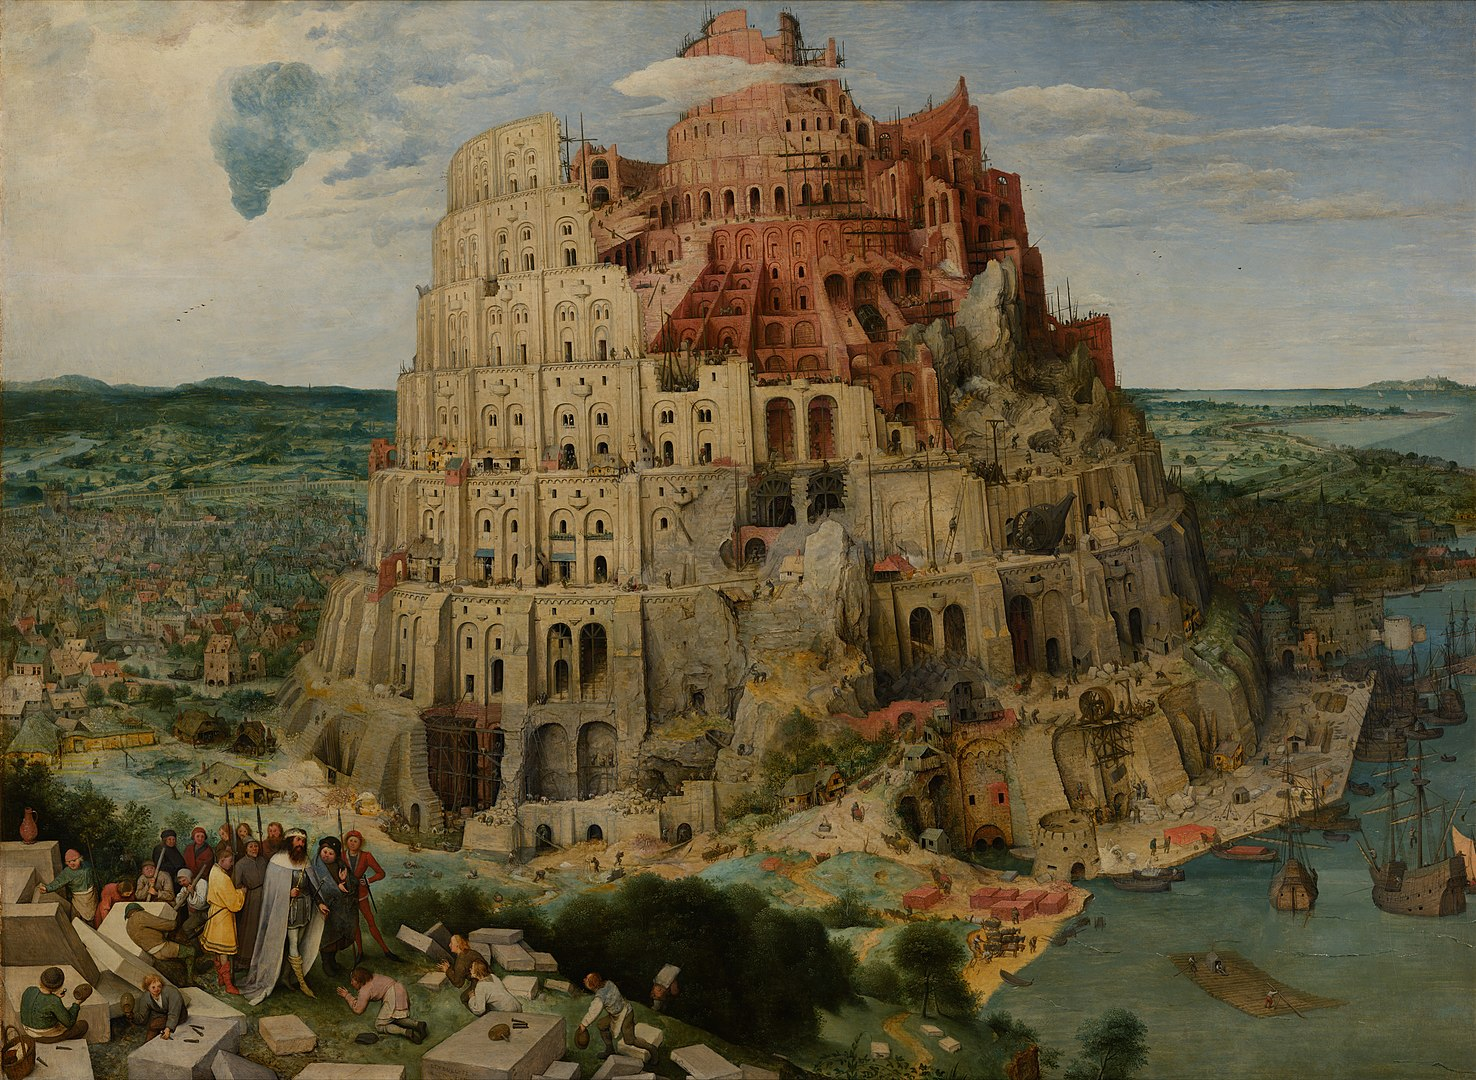
\includegraphics[width=1\linewidth]{111}
		\caption{\small\textit{\color{quantoan}Tháp Babel của Pieter Bruegel the Elder ($1563$), nguồn Wikipedia.}}
		\vspace*{-10pt}
	\end{figure}
	``Nhiều'' có thể gây rắc rối, còn ``vô hạn'' nói chung nguy hiểm. Ta hãy so sánh hai cách tư duy, chẳng hạn, để chứng minh rằng bình phương một số tự nhiên rồi thêm $1$ không bao giờ chia hết cho $3$.
	\vskip 0.1cm
	Hãy cho tôi một số tự nhiên, tôi sẽ chứng minh bình phương của nó rồi thêm $1$ không chia hết cho $3$!
	\vskip 0.1cm
	Đây giống như một lời thách thức của những nhà ảo thuật. Đưa thế nào là việc của bạn, chứng minh là việc của tôi.
	\vskip 0.1cm
	Quy nạp không như thế. Khi quy nạp tôi sẽ chỉ cho bạn thấy từng số, từng số một, khi bình phương lên, rồi thêm $1$ sẽ không thể chia hết cho $3$. 
	\vskip 0.1cm
	Điểm mấu chốt ở đây là, có vô hạn số tự nhiên, làm từng bước từng bước thế thì đến bao giờ?! Tới chỗ này, các nhà toán học quay trở lại lập luận ``cùn" nêu ở trên: cứ cho tôi một số cụ thể, thì thể nào tôi cũng sẽ đi đến. 
	\vskip 0.1cm
	Đây chính là cách các nhà toán học tiếp cận với vô hạn từ hữu hạn: tất cả là vô hạn nhưng từng cá thể là hữu hạn. 
	\vskip 0.1cm
	Ta hãy thử nhìn vấn đề từ một góc độ khác. Bây giờ sẽ không ai thách thức ai, mà tôi và bạn, chúng ta sẽ cùng suy nghĩ về việc chứng minh khẳng định trên bằng {\em phản chứng}. Phản chứng nghĩa là thay vì {\em chứng minh nó đúng}, ta sẽ chứng minh nó {\em không thể sai} -- như các bạn biết đó, toán học luôn đơn giản hóa mọi vấn đề, chỉ có thể đúng hoặc sai chứ không có khả năng nửa đúng nửa sai. 
	\vskip 0.1cm
	Để chứng minh nó không thể sai, ta sẽ đặt vấn đề nếu nó sai thì sao. Nếu mệnh đề trên sai, nghĩa là có số tự nhiên mà khi bình phương lên rồi thêm $1$ thì chia hết cho $3$.
	\vskip 0.1cm 
	Nếu có số như thế, thì sẽ có {\em số nhỏ nhất} trong chúng. Nếu ``số nhỏ nhất'' đó lớn hơn $3$, ta trừ nó đi $3$ đơn vị, số mới bình phương lên thêm $1$ vẫn chia hết cho $3$, vô lý vì số mới vẫn là số tự nhiên, lại bé hơn ``số nhỏ nhất''! Vậy ``số nhỏ nhất'' không quá $3$, nghĩa là $0$, $1$, hoặc $2$. Rõ ràng cả ba số này, khi bình phương lên thêm $1$ không chia hết cho $3$. Vô lý!
	\vskip 0.1cm
	Vô lý nghĩa khẳng định của chúng ta không thể sai. Vì không thể sai nên nó phải đúng. Nhắc lại là chỉ trong toán học, điều không sai mới là điều đúng các bạn nhé.
	\vskip 0.1cm
	Bản chất của vấn đề ở đây là gì? Các bạn hãy liên hệ với bài viết trước về tập hợp\footnote[2]{\color{quantoan}Xem ``Tự do trong Toán học'', Pi  Tập $6$, Số $5$, $2022$.}. Ở đây ta xét tập hợp những số tự nhiên mà khẳng định ``bình phương thêm $1$ chia hết cho $3$" đối với nó là SAI. Ta giả thiết phản chứng rằng tồn tại số như vậy, nghĩa là tập hợp này khác {\em rỗng}. Từ đó ta chọn số nhỏ nhất trong nó. Bản chất của vấn đề là sự tồn tại của số nhỏ nhất đó. Đây cũng là bản chất của phép quy nạp, và rộng hơn là bản chất của tập số tự nhiên: mọi tập hợp con khác rỗng đều chứa số nhỏ nhất.  
\end{multicols}